%!TeX root=../tese.tex
%("dica" para o editor de texto: este arquivo é parte de um documento maior)
% para saber mais: https://tex.stackexchange.com/q/78101

\chapter{Exemplos e dicas de \LaTeX{}}
\label{chap:exemplos}

Neste capítulo, apresentamos exemplos comuns com alguma complexidade e,
principalmente, pequenas dicas para evitar surpresas indesejáveis. Mesmo
que você já conheça \LaTeX{}, vale a pena analisar este material, incluindo
o código-fonte do capítulo. Se você ainda não conhece nada sobre \LaTeX{},
o Capítulo~\ref{chap:tutorial} e outros materiais citados na
Seção~\ref{sec:docs} apresentam os conceitos básicos.

\section{Bibliografia e referências}
\label{sec:exemplos-biblatex}

A documentação do pacote biblatex\index{biblatex}~\citep{biblatex} é
bastante extensa e explica (nas Seções~2.1.1 e 2.2.2) os diversos
tipos de documento suportados, bem como o significado de cada campo.
Na prática, às vezes é preciso fazer escolhas sobre
o que incluir na descrição de um item bibliográfico e muitas vezes
é mais fácil aprender copiando exemplos já existentes, como estes (consulte o
arquivo \texttt{bibliografia.bib} para ver como foi criado o banco de dados e a
bibliografia na página \pageref{sec:bib} para ver o resultado impresso):

\begin{multicols}{2}
  \begin{itemize}
    \item @Book: \cite{Knuth:96}.

    \item @Article (em periódico): \cite{floats2014}.

    \item @InProceedings (ou @Conference): \cite{alves03:simi}.

    \item @InCollection (capítulo de livro ou coletânea): \cite{bobaoglu93:concepts}.

    \item @PhdThesis: \cite{garcia01:PhD}.

    \item @MastersThesis: \cite{schmidt03:MSc}.

    \item @Techreport: \cite{alvisi99:analysisCIC}.

    \item @Manual: \cite{biblatex}.

    \item @Misc: \cite{gridftp}.

    \item @Online (para referência a artigo \emph{online}): \cite{fowler04:designDead}.

    \item @Online (para referência a página web): \cite{FSF:GNU-GPL}.
  \end{itemize}
\end{multicols}

A maioria das revistas científicas ainda utiliza bibtex e não
biblatex, mas isso não faz muita diferença na prática: \textsf{latexmk}
identifica automaticamente qual sistema usar durante a geração do
documento e os modelos normalmente já incluem os comandos
\textsf{\textbackslash{}bibliography},
\textsf{\textbackslash{}printbibliography},
\textsf{\textbackslash{}bibliographystyle} etc. conforme o caso.
O único detalhe importante se refere a datas:
\textsf{biblatex} prefere o uso do campo ``date'' para definir ano, mês
etc. No entanto, se você quiser garantir compatibilidade tanto com
\textsf{biblatex} quanto com \textsf{bibtex}, use os campos ``year'' e
``month''. Ambos reconhecem diversos formatos para o campo ``month'',
mas apenas um funciona corretamente com os dois: o nome do mês em inglês,
abreviado com três letras minúsculas e sem chaves, ou seja:

\begin{verbatim}
    ...
    author = {Fulano de Tal},
    year = {2011},
    month = oct,
    title = {Um título grandioso},
    ...
\end{verbatim}

Para citar material \emph{online}, há três casos:

\begin{itemize}
  \item Para citar publicações \emph{online} que se enquadram em
  formatos tradicionais (como um ebook ou a versão online de um artigo
  científico, independentemente de a revista existir ou não no formato
  impresso), use o tipo correspondente (\textsf{@article}, \textsf{@book},
  \textsf{@inproceedings} etc.) e acrescente o campo \textsf{url} no
  arquivo .bib, aceito por todos os tipos de documento do bibtex/biblatex.

  \item Para citar materiais essencialmente \emph{online} que possuem
  título e autor definidos (como uma postagem ou comentário em blog
  ou uma mensagem de email para uma lista de discussão), use o tipo
  \textsf{@online} de biblatex. Bibtex\index{bibtex}, por padrão,
  não tem um tipo específico para isso; com ele, normalmente usa-se
  o tipo ``misc'' e seu campo ``howpublished'' para especificar que
  se trata de um recurso \emph{online}.

  \item Se o que você quer citar não é propriamente uma ideia (que
  normalmente possui um autor e faz parte de um texto com título etc.)
  mas sim um sítio (como uma empresa, produto ou repositório de
  software), pode ser mais adequado colocar a referência apenas como
  nota de rodapé e não na lista de referências. Outra opção é criar
  uma segunda lista de referências especificamente para recursos
  \emph{online} desse tipo (biblatex\index{biblatex} permite criar
  múltiplas bibliografias).
\end{itemize}

\section{Identificando problemas}

Como mencionado na Seção~\ref{sec:limitations}, \LaTeX{} gera um grande
volume de mensagens informativas durante o processamento, o que torna mais
difícil encontrar problemas. O arquivo de configuração \cmd{latexmkrc} deste
modelo utiliza o programa \cmd{texlogsieve} para filtrar essas mensagens,
apresentando apenas as mais importantes para o usuário; considere usá-lo
em outros trabalhos com \LaTeX{} também.

\enlargethispage{\baselineskip}

\section{Modo matemático}\index{Modo matemático}

O modo matemático do \LaTeX{} tem sintaxe própria, mas ela não é complicada e
há bastante documentação \emph{online} a respeito. Por exemplo, ``massa e
energia são grandezas relacionadas pela Equação $E=mc^2$, definida inicialmente
por Einstein'', ou ainda ``equações de segundo grau (Equação \ref{eq:2grau})
são estudadas no ensino médio. As raízes de uma equação de segundo grau podem
ser encontradas por~\eqref{eq:bhaskara} --- a fórmula de Bháskara.
O valor do discriminante $\Delta$ (Equação \ref{eq:delta}) determina se a
equação tem zero, uma ou duas raízes reais~distintas''.

% Equação simples, com numeração à direita
\begin{equation}
  \label{eq:2grau}
  ax^2+bx+c=y \quad \forall x \in \mathbb{R}
\end{equation}

% Conjunto de equações agrupadas mas sem alinhamento, com numeração à direita
\begin{gather}
  \label{eq:bhaskara}
    y=0 \Leftrightarrow x=\frac{-b \pm \sqrt{\Delta}}{2a}
    \Leftrightarrow x \text{ é raiz da equação}\\
  \label{eq:delta}
    \Delta\enspace(\mathit{delta}) = b^2-4ac
\end{gather}

\enlargethispage{\baselineskip}

Para inserir um espaço explicitamente no modo matemático, use
\ltxcmd{quad} ou \ltxcmd{enspace}. Para inserir texto ``normal'' em
uma fórmula matemática, use \ltxcmd{text\{texto\}} (para texto de fato)
ou \ltxcmd{mathit\{texto\}} (para nomes de variáveis ou funções com
mais de uma letra). Pode ser necessário deixar um espaço no início do
texto para evitar que ele fique colado com o caractere matemático que
o antecede.

Para recursos mais sofisticados, incluindo frações com múltiplas linhas,
matrizes, sistemas de equações alinhadas, setas, acentos etc., procure
a documentação das packages \textsf{amsmath} e \textsf{mathtools}. Para
teoremas, lemas, conjecturas etc., leia a documentação das packages
\textsf{amsthm} e \textsf{thmtools} e decida de quais tipos de estrutura
você vai precisar no seu documento. Aqui criamos três: ``Pegadinha'',
``Teorema'' e ``Conjectura'' (observe as numerações):\looseness=-1

% A aparência dos teoremas/lemas/etc. é definida por estilos. Há três
% estilos padrão (plain, definition e remark), mas é possível criar outros:
\newtheoremstyle{smile} % nome do estilo
{3pt} % espaço antes
{3pt} % espaço depois
{\itshape} % fonte do corpo
{} % Indentação
{\bfseries} % fonte do título
{} % pontuação após o título
{.5em} % espaço após o título
{\thmname{#1}\thmnumber{ #2}\thmnote{ (#3)} :-)\space} % formato do título
% vazio significa {\thmname{#1}\thmnumber{ #2}\thmnote{ (#3)}}

\newtheoremstyle{maybe} % nome do estilo
{3pt} % espaço antes
{3pt} % espaço depois
{\itshape} % fonte do corpo
{} % Indentação
{\bfseries} % fonte do título
{:} % pontuação após o título
{.5em} % espaço após o título
{\thmname{#1}\space(?)\thmnumber{ #2}\thmnote{ (#3)}} % formato do título
% vazio significa {\thmname{#1}\thmnumber{ #2}\thmnote{ (#3)}}

\theoremstyle{smile} % As próximas definições usam este estilo
\newtheorem{absurd}{Pegadinha}

\begin{absurd}\label{thm:doisum}
  $1=0$
\end{absurd}

% "proof" é pré-definido por amsthm
\begin{proof}
Tomemos dois números, $a$ e $b$, tais que $a=b+1$.

% Múltiplas linhas alinhadas em "&", sem numeração
\begin{displaymath}
  \begin{split}
    a &= b+1 \\
    (a-b)a &= (a-b)(b+1) \\
    a^2 - ab &= ab + a -b^2 -b \\
    a^2 -ab -a &= ab -b^2 -b \\
    a(a-b-1) &= b(a-b-1) \\
    a \cancel{(a-b-1)} &= b \cancel{(a-b-1)} \\
    a &= b \\
    b+1 &= b \\
    1 &= b-b \\
    1 &= 0
  \end{split}
\end{displaymath}
\end{proof}

\theoremstyle{plain} % As próximas definições usam este estilo
\newtheorem{theorem}{Teorema}

\begin{theorem}
  \label{thm:graphcolor}
  É sempre possível colorir os vértices de um grafo sem que dois vértices
  adjacentes tenham a mesma cor usando no máximo quatro cores diferentes.
\end{theorem}

\begin{proof}
  A demonstração do Teorema~\ref{thm:graphcolor} é um exercício
  a cargo do leitor.
  % Como isto não é de fato uma prova, queremos eliminar o símbolo
  % "QED" que o ambiente proof acrescenta automaticamente.
  \renewcommand\qedsymbol{} % tem efeito apenas nesta prova!
\end{proof}

\theoremstyle{maybe} % As próximas definições usam este estilo
\newtheorem{conjecture}{Conjectura}

\begin{conjecture}
  \label{conj:fermat}
  Dado qualquer inteiro $n > 2$, não existem inteiros positivos
  $a$, $b$ e $c$ tais que $a^n + b^n = c^n$.
\end{conjecture}

\begin{proof}
  Este espaço é muito pequeno para apresentá-la.
  \renewcommand\qedsymbol{}
\end{proof}

\begin{theorem}
  \label{thm:pnp}
  \textup{\textsf{\textbf{P$\ne$NP}}}
\end{theorem}

\begin{proof}
  \textsf{\textbf{P}} tem apenas uma letra, enquanto
  \textsf{\textbf{NP}} tem duas letras.
\end{proof}


\section{Quebras de página}
\label{sec:quebras}

O algoritmo que \LaTeX{} usa para quebrar páginas funciona bem, minimizando
linhas órfãs ou viúvas e garantindo uma distribuição homogênea do texto na
página, mas não é excelente. Assim, se houver quebras de página ruins no
seu texto final, pode ser útil modificá-las manualmente. Uma técnica usada
por editores profissionais é mudar ligeiramente a altura do texto impresso
em algumas páginas, melhorando a distribuição geral do texto. Para isso,
ao invés de comandos como \ltxcmd{pagebreak} ou \ltxcmd{newpage}, o mais
adequado é usar \ltxcmd{enlargethispage\{\sla{}baselineskip\}} (ou
\cmd{-1\sla{}baselineskip}). Esse comando instrui \LaTeX{} a fazer a
página ligeiramente maior (ou menor), tornando possível acomodar mais
uma linha de texto (ou uma linha a menos). Em documentos frente e verso,
lembre-se de sempre garantir que a página adjacente também tenha seu
tamanho modificado para que a alteração não seja tão perceptível. Um
outro truque às vezes útil é aplicar o comando \ltxcmd{looseness=1} (ou
-1) a um parágrafo, que faz \LaTeX{} tentar reorganizar as quebras de
linha de maneira a fazer o parágrafo ter uma linha a mais (ou a menos),
se isso for possível.

\section{Figuras, gráficos e outros \emph{floats}}\index{Floats}
\label{sec:exemplos-graficos}

Evidentemente, \LaTeX{} permite inserir figuras no texto; além disso, ele
também permite girá-las e criar subfiguras (com sublegendas\index{Legendas}),
como no exemplo da Figura~\ref{fig:subfigures}\index{Subfiguras}, que inclui
as subfiguras~\ref{fig:subfigures:a} e~\ref{fig:subfigures:b}.

% As packages relevantes para lidar com figuras são graphicx,
% float, caption, rotating e subcaption. Observe que "subfigure"
% e "subtable" são definidos na package subcaption, *não* na
% package subfigure! A package subfigure é obsoleta.

%%%%%%%%% Figuras lado-a-lado %%%%%%%%%
\begin{figure}
  \centering

  \begin{subfigure}{0.4\textwidth}
    \centering
    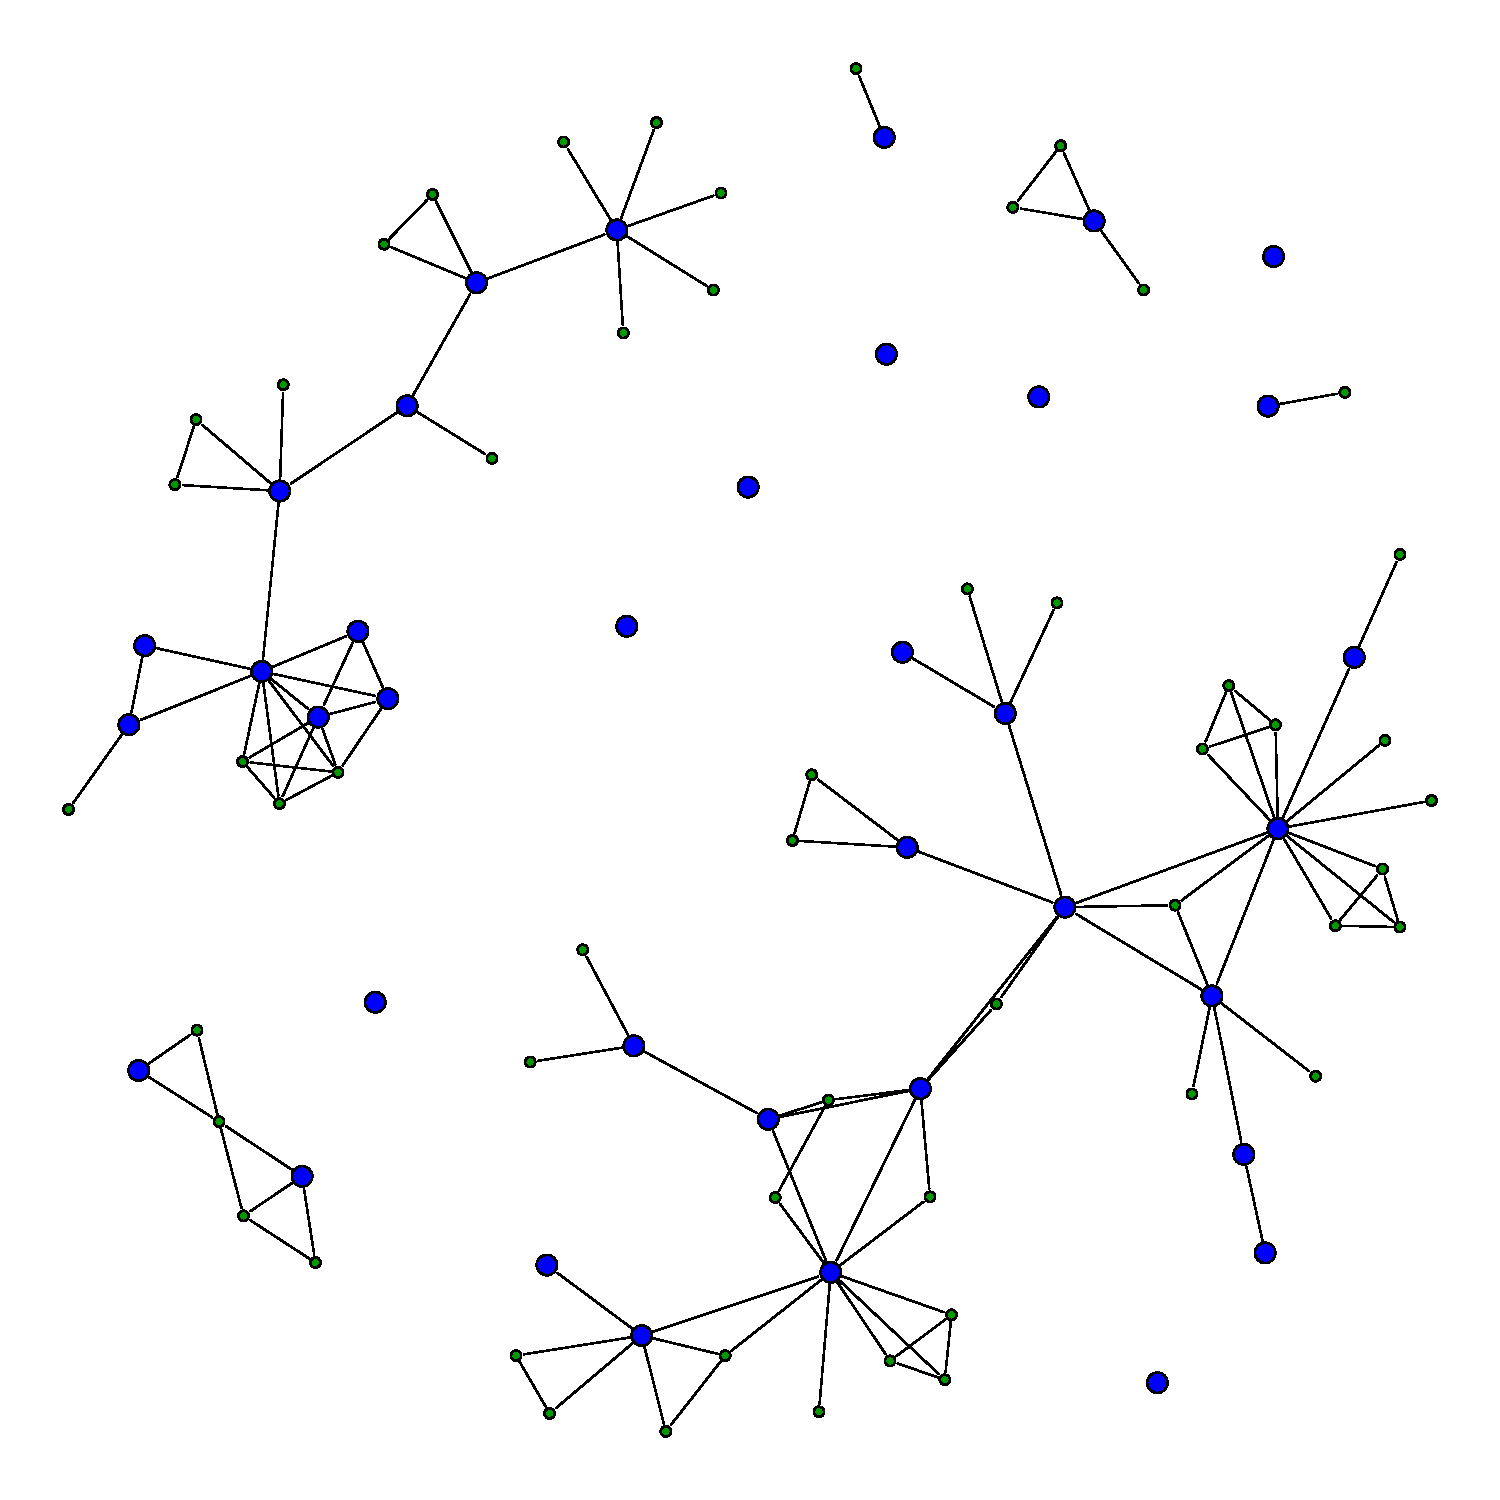
\includegraphics[width=.8\textwidth]{exemplo-grafo}
    \caption{Uma figura simples.\label{fig:subfigures:a}}
  \end{subfigure}
  % ATENÇÃO: Se você deixar uma linha em branco entre as subfiguras,
  % LaTeX vai considerar que cada uma delas pertence a um "parágrafo"
  % diferente e, portanto, vai colocá-las em linhas separadas ao invés
  % de lado a lado.
  \begin{subfigure}{0.4\textwidth}
    \centering
    \begin{turn}{90} % package rotating
      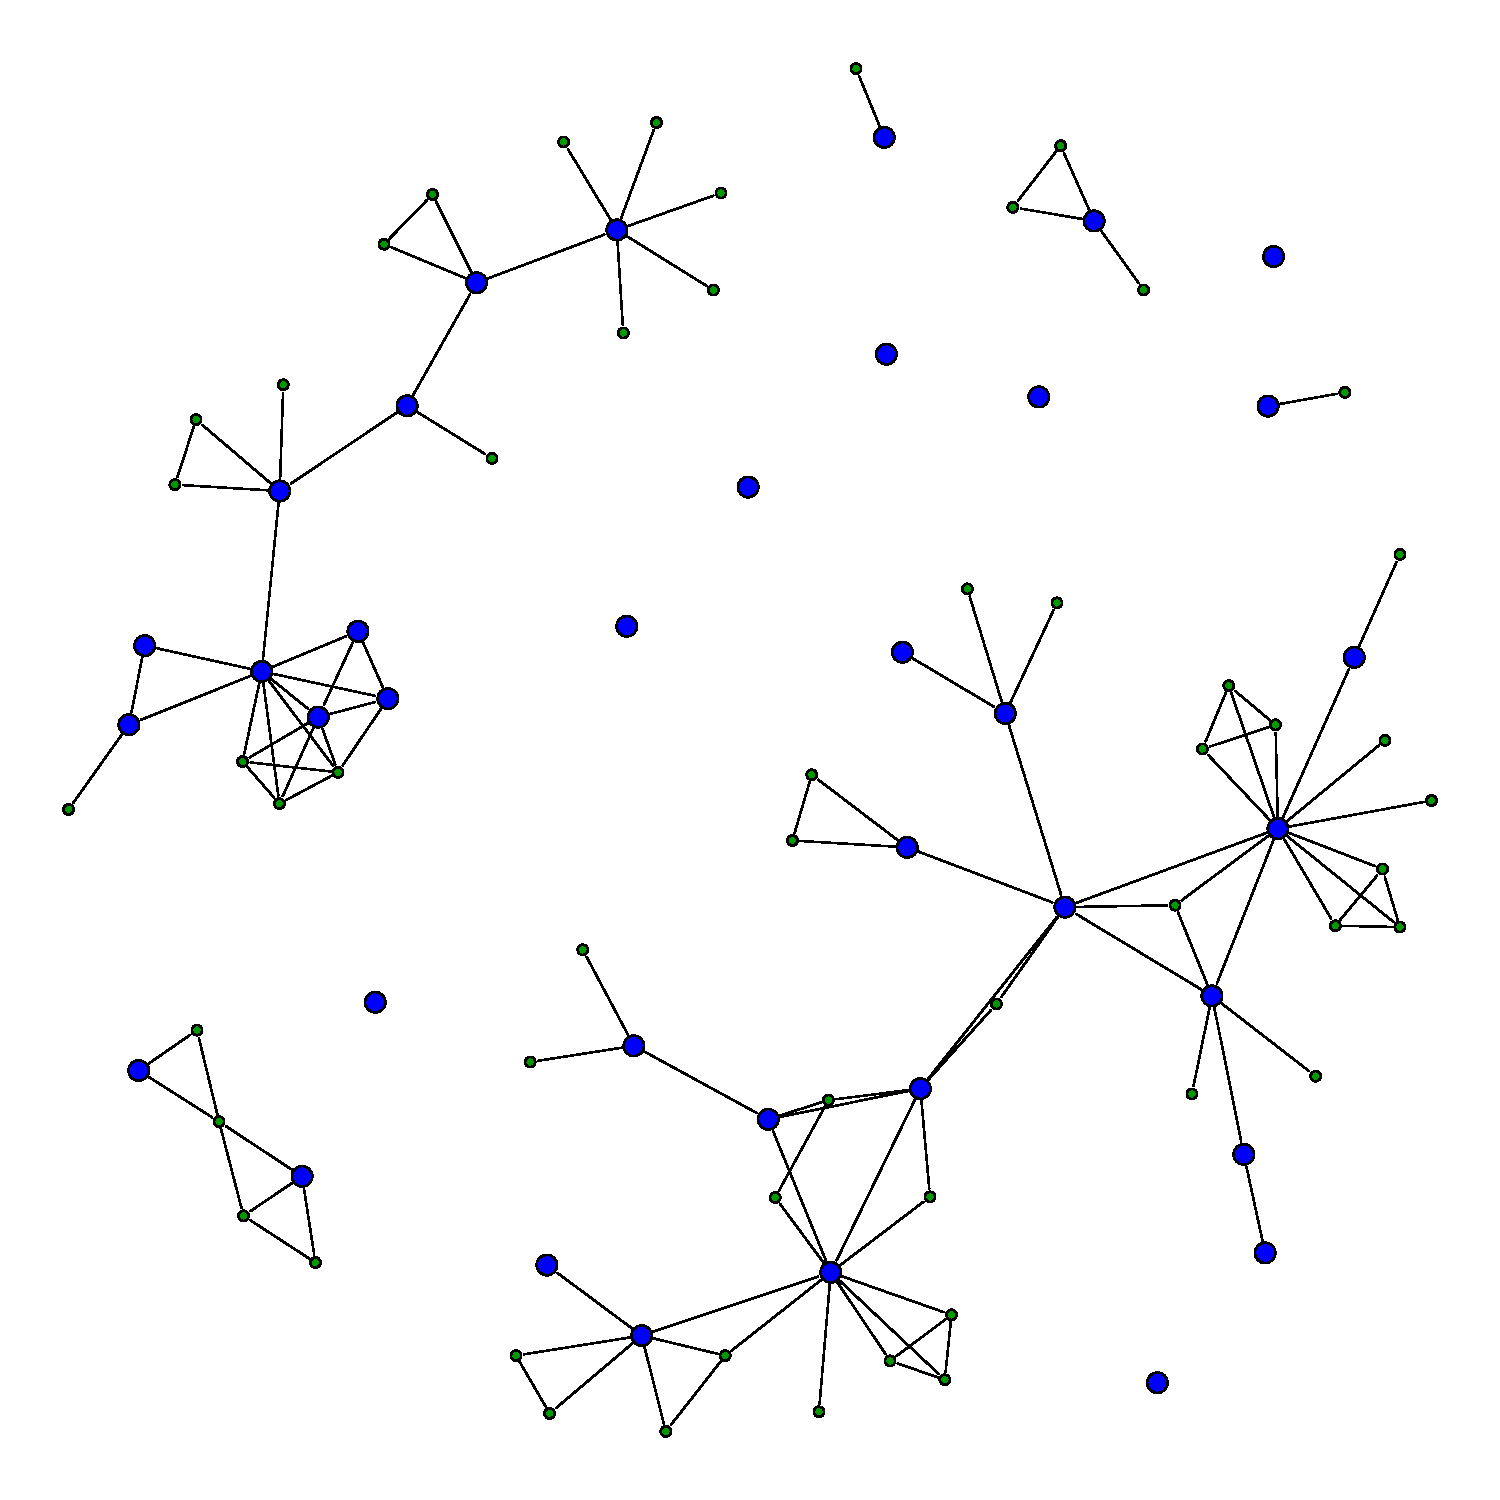
\includegraphics[width=.8\textwidth]{exemplo-grafo}
    \end{turn}
    \caption{O mesmo exemplo, girado.\label{fig:subfigures:b}}
  \end{subfigure}

  \caption{Exemplo de subfiguras.\label{fig:subfigures}}
\end{figure}

\emph{Floats} em geral incluem uma legenda e um \emph{label}.
Prefira sempre colocar o comando \textsf{\textbackslash{}label} de uma
figura ou tabela dentro do comando \textsf{\textbackslash{}caption};
não fazê-lo muitas vezes funciona, mas às vezes causa problemas.

Você pode carregar arquivos de imagem de um subdiretório usando
\texttt{dir/img.pdf}, mas é mais fácil modificar o comando
\textsf{\textbackslash{}graphicspath} próximo ao início de cada
arquivo~\texttt{.tex} de exemplo.

Para centralizar uma imagem mais larga que o texto da página, use
a \emph{package} \textsf{adjustbox} (incluída neste modelo):

\begin{verbatim}
  \begin{figure}
  \adjustbox{center}{\includegraphics[width=1.2\textwidth]{img.pdf}}
  \caption{...}
  \end{figure}
\end{verbatim}

Uma ``figura'', na verdade, pode ser qualquer tipo de conteúdo ilustrativo
(um exemplo interessante é o cronograma mostrado na Figura~\ref{fig:gantt})
mas, com a \textit{package} \textsf{float}, também é possível definir ambientes
específicos para cada tipo de conteúdo adicional (cada um com numeração
independente), como é o caso do Programa~\ref{prog:java}\index{Floats}. Há
mais informações e dicas sobre recursos específicos para inclusão de
código-fonte e pseudocódigo no Anexo\linebreak\ref{ap:pseudocode}\footnote{
Observe que o nome do Anexo (``\ref{ap:pseudocode}'') foi impresso em
uma linha separada, o que não é muito bom visualmente. Para evitar que isso
aconteça (não só no final do parágrafo, mas em qualquer quebra de linha),
utilize um espaço não-separável para fazer referências a figuras, tabelas,
seções etc. ou antes de símbolos: ``\textsf{\dots no
Anexo\textasciitilde\textbackslash{}ref\{ap:pseudocode\}}'',
``\textsf{O discriminante é denotado
por\textasciitilde{}\$\textbackslash{}Delta\$}''.}.

%%%%%%% Cronograma %%%%%%%

\begin{figure}
  \centering

  % Package pgfgantt; veja o arquivo imegoodies.sty, em que vários
  % aspectos da aparência deste diagrama foram definidos.
  \begin{ganttchart}[
                     time slot format=isodate-yearmonth,
                     time slot unit=month,
                    ]{2017-11}{2018-5}

    \gantttitlecalendar{year,month=shortname} \ganttnewline

    \ganttgroup[progress=45]{Experimento}{2017-11}{2018-2} \ganttnewline
    \ganttbar[progress=100]{
      Preparação\ganttalignnewline
      (compra de insumos)
      }{2017-11}{2017-12} \ganttnewline
    \ganttbar[progress=30]{Execução}{2017-12}{2018-1} \ganttnewline
    \ganttbar[progress=0]{Análise}{2017-12}{2018-2} \ganttnewline

    \ganttgroup[progress=0]{Artigo}{2018-1}{2018-4} \ganttnewline
    \ganttbar[progress=0]{Escrita}{2018-1}{2018-3} \ganttnewline
    \ganttbar[progress=0]{Revisão}{2018-3}{2018-4} \ganttnewline

    \ganttmilestone{Submissão}{2018-4}
  \end{ganttchart}

  \caption{Exemplo de cronograma.\label{fig:gantt}}
\end{figure}

%%%%%%%% Código fonte %%%%%%%%

% Foi utilizado o pacote listings para formatar o código fonte.
% Veja os parâmetros de configuração no arquivo source-code.tex.
\begin{program}
  \index{Java}
  \centering

\begin{lstlisting}[language=Java, style=wider]
  for (i = 0; i < 20; i++)
  {
      // Comentário
      System.out.println("Mensagem...");
  }
\end{lstlisting}

  \caption{Exemplo de laço em Java.\label{prog:java}}
\end{program}

%%%%%

\LaTeX{} também é capaz de gerar ilustrações e diagramas diretamente, mas
usar esses recursos em geral não é trivial. Em particular, a package
\textsf{tikz} oferece bons mecanismos para a criação de figuras (incluindo
funções pré-prontas para formas geométricas, grafos, matrizes etc.) e é
fácil usá-la para traçar linhas ou curvas simples.

Gráficos de dados ou funções matemáticas de excelente qualidade podem ser
gerados com a \textit{package} \pkg{pgfplots} (há um exemplo comentado neste
arquivo; experimente des-comentar para ver o resultado). Também é possível
importar gráficos gerados por \cmd{matplotlib}, \cmd{gnuplot} e \cmd{R}
como qualquer outra imagem, mas nesse caso a fonte usada nesses gráficos
provavelmente será diferente do corpo do texto. Felizmente, isso pode ser
solucionado: \cmd{Gnuplot} (com o \emph{driver} \cmd{lua tikz}\footnote{
\url{gnuplot.info/docs_5.5/loc20850.html}}),
\cmd{matplotlib} (com o \emph{backend} \textsc{pgf}\footnote{\url
{matplotlib.org/users/pgf.html}})
e \cmd{R} (com \cmd{tikzDevice}\footnote{\url
{cran.r-project.org/package=tikzDevice}}) são capazes de exportar gráficos de
dados na forma de comandos para \pkg{tikz}\footnote{Você pode se interessar
também pela \textit{package} \texttt{gnuplottex}.}: o resultado pode ser
visto na Figura~\ref{fig:graficos}.

\begin{figure}
  \centering
  \begin{subfigure}[b]{.45\textwidth}
    \input{figuras/gnuplot.tkz} % Exemplo com gnuplot
    %\begin{tikzpicture}
  \sffamily\scriptsize
  \begin{axis}[
    width=2.9in, height=1.9in,
    %title=Algum título,
    ylabel=$f(x)$,
    xlabel=$x$,
    xmin = 1,
    ymin = 0,
    xmax = 12.5,
    ymax = 145,
    ytick distance = 25,
    legend pos = north west,
    legend cell align = left,
  ]

  \addlegendentry{$10x-10$}
  \addplot+ [no marks] table
  {
     1.0   0
     2.0  10
     5.0  40
     7.0  60
    10.0  90
    11.9 109
  };

  \addlegendentry{$x^2-1$}
  \addplot+ [mark = +] table
  {
     1.0   0.0
     2.0   3.0
     3.0   8.0
     4.0  15.0
     6.0  35.0
     8.0  63.0
    11.9 140.6
  };
  \addlegendentry{$25\log_{2}(x)$}
  \addplot+ [error bars/y dir=both, error bars/y explicit,]
      table [y error minus index=2, y error plus index=3,]
  {
     1.0  0.00 0.0 0.0
     1.5 14.62 3.1 6.8
     2.0 25.00 5.3 3.8
     3.0 39.62 3.7 6.2
     5.0 58.05 2.2 5.5
     7.0 70.18 3.9 6.6
     8.0 75.00 7.9 2.3
    11.9 89.32 7.9 3.8
  };
  \end{axis}
\end{tikzpicture}
 % Exemplo com pgfplots
    \caption{\texttt{gnuplot}.\label{fig:gnuplot}}
  \end{subfigure}
  \begin{subfigure}[b]{.5\textwidth}
    %% Creator: Matplotlib, PGF backend
%%
%% To include the figure in your LaTeX document, write
%%   \input{<filename>.pgf}
%%
%% Make sure the required packages are loaded in your preamble
%%   \usepackage{pgf}
%%
%% and, on pdftex
%%   \usepackage[utf8]{inputenc}\DeclareUnicodeCharacter{2212}{-}
%%
%% or, on luatex and xetex
%%   \usepackage{unicode-math}
%%
%% Figures using additional raster images can only be included by \input if
%% they are in the same directory as the main LaTeX file. For loading figures
%% from other directories you can use the `import` package
%%   \usepackage{import}
%%
%% and then include the figures with
%%   \import{<path to file>}{<filename>.pgf}
%%
%% Matplotlib used the following preamble
%%   \usepackage{fontspec}
%%   \setmainfont{DejaVuSerif.ttf}[Path=/usr/share/matplotlib/mpl-data/fonts/ttf/]
%%   \setsansfont{DejaVuSans.ttf}[Path=/usr/share/matplotlib/mpl-data/fonts/ttf/]
%%   \setmonofont{DejaVuSansMono.ttf}[Path=/usr/share/matplotlib/mpl-data/fonts/ttf/]
%%
\begingroup%
\makeatletter%
\begin{pgfpicture}%
\pgfpathrectangle{\pgfpointorigin}{\pgfqpoint{2.900000in}{1.800000in}}%
\pgfusepath{use as bounding box, clip}%
\begin{pgfscope}%
\pgfsetbuttcap%
\pgfsetmiterjoin%
\definecolor{currentfill}{rgb}{1.000000,1.000000,1.000000}%
\pgfsetfillcolor{currentfill}%
\pgfsetlinewidth{0.000000pt}%
\definecolor{currentstroke}{rgb}{1.000000,1.000000,1.000000}%
\pgfsetstrokecolor{currentstroke}%
\pgfsetdash{}{0pt}%
\pgfpathmoveto{\pgfqpoint{0.000000in}{0.000000in}}%
\pgfpathlineto{\pgfqpoint{2.900000in}{0.000000in}}%
\pgfpathlineto{\pgfqpoint{2.900000in}{1.800000in}}%
\pgfpathlineto{\pgfqpoint{0.000000in}{1.800000in}}%
\pgfpathclose%
\pgfusepath{fill}%
\end{pgfscope}%
\begin{pgfscope}%
\pgfsetbuttcap%
\pgfsetmiterjoin%
\definecolor{currentfill}{rgb}{1.000000,1.000000,1.000000}%
\pgfsetfillcolor{currentfill}%
\pgfsetlinewidth{0.000000pt}%
\definecolor{currentstroke}{rgb}{0.000000,0.000000,0.000000}%
\pgfsetstrokecolor{currentstroke}%
\pgfsetstrokeopacity{0.000000}%
\pgfsetdash{}{0pt}%
\pgfpathmoveto{\pgfqpoint{0.616528in}{0.472778in}}%
\pgfpathlineto{\pgfqpoint{2.780000in}{0.472778in}}%
\pgfpathlineto{\pgfqpoint{2.780000in}{1.680000in}}%
\pgfpathlineto{\pgfqpoint{0.616528in}{1.680000in}}%
\pgfpathclose%
\pgfusepath{fill}%
\end{pgfscope}%
\begin{pgfscope}%
\pgfsetbuttcap%
\pgfsetroundjoin%
\definecolor{currentfill}{rgb}{0.000000,0.000000,0.000000}%
\pgfsetfillcolor{currentfill}%
\pgfsetlinewidth{0.803000pt}%
\definecolor{currentstroke}{rgb}{0.000000,0.000000,0.000000}%
\pgfsetstrokecolor{currentstroke}%
\pgfsetdash{}{0pt}%
\pgfsys@defobject{currentmarker}{\pgfqpoint{0.000000in}{-0.048611in}}{\pgfqpoint{0.000000in}{0.000000in}}{%
\pgfpathmoveto{\pgfqpoint{0.000000in}{0.000000in}}%
\pgfpathlineto{\pgfqpoint{0.000000in}{-0.048611in}}%
\pgfusepath{stroke,fill}%
}%
\begin{pgfscope}%
\pgfsys@transformshift{0.804656in}{0.472778in}%
\pgfsys@useobject{currentmarker}{}%
\end{pgfscope}%
\end{pgfscope}%
\begin{pgfscope}%
\definecolor{textcolor}{rgb}{0.000000,0.000000,0.000000}%
\pgfsetstrokecolor{textcolor}%
\pgfsetfillcolor{textcolor}%
\pgftext[x=0.804656in,y=0.375556in,,top]{\color{textcolor}\sffamily\fontsize{8.000000}{9.600000}\selectfont 2}%
\end{pgfscope}%
\begin{pgfscope}%
\pgfsetbuttcap%
\pgfsetroundjoin%
\definecolor{currentfill}{rgb}{0.000000,0.000000,0.000000}%
\pgfsetfillcolor{currentfill}%
\pgfsetlinewidth{0.803000pt}%
\definecolor{currentstroke}{rgb}{0.000000,0.000000,0.000000}%
\pgfsetstrokecolor{currentstroke}%
\pgfsetdash{}{0pt}%
\pgfsys@defobject{currentmarker}{\pgfqpoint{0.000000in}{-0.048611in}}{\pgfqpoint{0.000000in}{0.000000in}}{%
\pgfpathmoveto{\pgfqpoint{0.000000in}{0.000000in}}%
\pgfpathlineto{\pgfqpoint{0.000000in}{-0.048611in}}%
\pgfusepath{stroke,fill}%
}%
\begin{pgfscope}%
\pgfsys@transformshift{1.180912in}{0.472778in}%
\pgfsys@useobject{currentmarker}{}%
\end{pgfscope}%
\end{pgfscope}%
\begin{pgfscope}%
\definecolor{textcolor}{rgb}{0.000000,0.000000,0.000000}%
\pgfsetstrokecolor{textcolor}%
\pgfsetfillcolor{textcolor}%
\pgftext[x=1.180912in,y=0.375556in,,top]{\color{textcolor}\sffamily\fontsize{8.000000}{9.600000}\selectfont 4}%
\end{pgfscope}%
\begin{pgfscope}%
\pgfsetbuttcap%
\pgfsetroundjoin%
\definecolor{currentfill}{rgb}{0.000000,0.000000,0.000000}%
\pgfsetfillcolor{currentfill}%
\pgfsetlinewidth{0.803000pt}%
\definecolor{currentstroke}{rgb}{0.000000,0.000000,0.000000}%
\pgfsetstrokecolor{currentstroke}%
\pgfsetdash{}{0pt}%
\pgfsys@defobject{currentmarker}{\pgfqpoint{0.000000in}{-0.048611in}}{\pgfqpoint{0.000000in}{0.000000in}}{%
\pgfpathmoveto{\pgfqpoint{0.000000in}{0.000000in}}%
\pgfpathlineto{\pgfqpoint{0.000000in}{-0.048611in}}%
\pgfusepath{stroke,fill}%
}%
\begin{pgfscope}%
\pgfsys@transformshift{1.557168in}{0.472778in}%
\pgfsys@useobject{currentmarker}{}%
\end{pgfscope}%
\end{pgfscope}%
\begin{pgfscope}%
\definecolor{textcolor}{rgb}{0.000000,0.000000,0.000000}%
\pgfsetstrokecolor{textcolor}%
\pgfsetfillcolor{textcolor}%
\pgftext[x=1.557168in,y=0.375556in,,top]{\color{textcolor}\sffamily\fontsize{8.000000}{9.600000}\selectfont 6}%
\end{pgfscope}%
\begin{pgfscope}%
\pgfsetbuttcap%
\pgfsetroundjoin%
\definecolor{currentfill}{rgb}{0.000000,0.000000,0.000000}%
\pgfsetfillcolor{currentfill}%
\pgfsetlinewidth{0.803000pt}%
\definecolor{currentstroke}{rgb}{0.000000,0.000000,0.000000}%
\pgfsetstrokecolor{currentstroke}%
\pgfsetdash{}{0pt}%
\pgfsys@defobject{currentmarker}{\pgfqpoint{0.000000in}{-0.048611in}}{\pgfqpoint{0.000000in}{0.000000in}}{%
\pgfpathmoveto{\pgfqpoint{0.000000in}{0.000000in}}%
\pgfpathlineto{\pgfqpoint{0.000000in}{-0.048611in}}%
\pgfusepath{stroke,fill}%
}%
\begin{pgfscope}%
\pgfsys@transformshift{1.933424in}{0.472778in}%
\pgfsys@useobject{currentmarker}{}%
\end{pgfscope}%
\end{pgfscope}%
\begin{pgfscope}%
\definecolor{textcolor}{rgb}{0.000000,0.000000,0.000000}%
\pgfsetstrokecolor{textcolor}%
\pgfsetfillcolor{textcolor}%
\pgftext[x=1.933424in,y=0.375556in,,top]{\color{textcolor}\sffamily\fontsize{8.000000}{9.600000}\selectfont 8}%
\end{pgfscope}%
\begin{pgfscope}%
\pgfsetbuttcap%
\pgfsetroundjoin%
\definecolor{currentfill}{rgb}{0.000000,0.000000,0.000000}%
\pgfsetfillcolor{currentfill}%
\pgfsetlinewidth{0.803000pt}%
\definecolor{currentstroke}{rgb}{0.000000,0.000000,0.000000}%
\pgfsetstrokecolor{currentstroke}%
\pgfsetdash{}{0pt}%
\pgfsys@defobject{currentmarker}{\pgfqpoint{0.000000in}{-0.048611in}}{\pgfqpoint{0.000000in}{0.000000in}}{%
\pgfpathmoveto{\pgfqpoint{0.000000in}{0.000000in}}%
\pgfpathlineto{\pgfqpoint{0.000000in}{-0.048611in}}%
\pgfusepath{stroke,fill}%
}%
\begin{pgfscope}%
\pgfsys@transformshift{2.309680in}{0.472778in}%
\pgfsys@useobject{currentmarker}{}%
\end{pgfscope}%
\end{pgfscope}%
\begin{pgfscope}%
\definecolor{textcolor}{rgb}{0.000000,0.000000,0.000000}%
\pgfsetstrokecolor{textcolor}%
\pgfsetfillcolor{textcolor}%
\pgftext[x=2.309680in,y=0.375556in,,top]{\color{textcolor}\sffamily\fontsize{8.000000}{9.600000}\selectfont 10}%
\end{pgfscope}%
\begin{pgfscope}%
\pgfsetbuttcap%
\pgfsetroundjoin%
\definecolor{currentfill}{rgb}{0.000000,0.000000,0.000000}%
\pgfsetfillcolor{currentfill}%
\pgfsetlinewidth{0.803000pt}%
\definecolor{currentstroke}{rgb}{0.000000,0.000000,0.000000}%
\pgfsetstrokecolor{currentstroke}%
\pgfsetdash{}{0pt}%
\pgfsys@defobject{currentmarker}{\pgfqpoint{0.000000in}{-0.048611in}}{\pgfqpoint{0.000000in}{0.000000in}}{%
\pgfpathmoveto{\pgfqpoint{0.000000in}{0.000000in}}%
\pgfpathlineto{\pgfqpoint{0.000000in}{-0.048611in}}%
\pgfusepath{stroke,fill}%
}%
\begin{pgfscope}%
\pgfsys@transformshift{2.685936in}{0.472778in}%
\pgfsys@useobject{currentmarker}{}%
\end{pgfscope}%
\end{pgfscope}%
\begin{pgfscope}%
\definecolor{textcolor}{rgb}{0.000000,0.000000,0.000000}%
\pgfsetstrokecolor{textcolor}%
\pgfsetfillcolor{textcolor}%
\pgftext[x=2.685936in,y=0.375556in,,top]{\color{textcolor}\sffamily\fontsize{8.000000}{9.600000}\selectfont 12}%
\end{pgfscope}%
\begin{pgfscope}%
\definecolor{textcolor}{rgb}{0.000000,0.000000,0.000000}%
\pgfsetstrokecolor{textcolor}%
\pgfsetfillcolor{textcolor}%
\pgftext[x=1.698264in,y=0.212470in,,top]{\color{textcolor}\sffamily\fontsize{8.000000}{9.600000}\selectfont \(\displaystyle x\)}%
\end{pgfscope}%
\begin{pgfscope}%
\pgfsetbuttcap%
\pgfsetroundjoin%
\definecolor{currentfill}{rgb}{0.000000,0.000000,0.000000}%
\pgfsetfillcolor{currentfill}%
\pgfsetlinewidth{0.803000pt}%
\definecolor{currentstroke}{rgb}{0.000000,0.000000,0.000000}%
\pgfsetstrokecolor{currentstroke}%
\pgfsetdash{}{0pt}%
\pgfsys@defobject{currentmarker}{\pgfqpoint{-0.048611in}{0.000000in}}{\pgfqpoint{-0.000000in}{0.000000in}}{%
\pgfpathmoveto{\pgfqpoint{-0.000000in}{0.000000in}}%
\pgfpathlineto{\pgfqpoint{-0.048611in}{0.000000in}}%
\pgfusepath{stroke,fill}%
}%
\begin{pgfscope}%
\pgfsys@transformshift{0.616528in}{0.472778in}%
\pgfsys@useobject{currentmarker}{}%
\end{pgfscope}%
\end{pgfscope}%
\begin{pgfscope}%
\definecolor{textcolor}{rgb}{0.000000,0.000000,0.000000}%
\pgfsetstrokecolor{textcolor}%
\pgfsetfillcolor{textcolor}%
\pgftext[x=0.448613in, y=0.430569in, left, base]{\color{textcolor}\sffamily\fontsize{8.000000}{9.600000}\selectfont 0}%
\end{pgfscope}%
\begin{pgfscope}%
\pgfsetbuttcap%
\pgfsetroundjoin%
\definecolor{currentfill}{rgb}{0.000000,0.000000,0.000000}%
\pgfsetfillcolor{currentfill}%
\pgfsetlinewidth{0.803000pt}%
\definecolor{currentstroke}{rgb}{0.000000,0.000000,0.000000}%
\pgfsetstrokecolor{currentstroke}%
\pgfsetdash{}{0pt}%
\pgfsys@defobject{currentmarker}{\pgfqpoint{-0.048611in}{0.000000in}}{\pgfqpoint{-0.000000in}{0.000000in}}{%
\pgfpathmoveto{\pgfqpoint{-0.000000in}{0.000000in}}%
\pgfpathlineto{\pgfqpoint{-0.048611in}{0.000000in}}%
\pgfusepath{stroke,fill}%
}%
\begin{pgfscope}%
\pgfsys@transformshift{0.616528in}{0.680920in}%
\pgfsys@useobject{currentmarker}{}%
\end{pgfscope}%
\end{pgfscope}%
\begin{pgfscope}%
\definecolor{textcolor}{rgb}{0.000000,0.000000,0.000000}%
\pgfsetstrokecolor{textcolor}%
\pgfsetfillcolor{textcolor}%
\pgftext[x=0.377921in, y=0.638710in, left, base]{\color{textcolor}\sffamily\fontsize{8.000000}{9.600000}\selectfont 25}%
\end{pgfscope}%
\begin{pgfscope}%
\pgfsetbuttcap%
\pgfsetroundjoin%
\definecolor{currentfill}{rgb}{0.000000,0.000000,0.000000}%
\pgfsetfillcolor{currentfill}%
\pgfsetlinewidth{0.803000pt}%
\definecolor{currentstroke}{rgb}{0.000000,0.000000,0.000000}%
\pgfsetstrokecolor{currentstroke}%
\pgfsetdash{}{0pt}%
\pgfsys@defobject{currentmarker}{\pgfqpoint{-0.048611in}{0.000000in}}{\pgfqpoint{-0.000000in}{0.000000in}}{%
\pgfpathmoveto{\pgfqpoint{-0.000000in}{0.000000in}}%
\pgfpathlineto{\pgfqpoint{-0.048611in}{0.000000in}}%
\pgfusepath{stroke,fill}%
}%
\begin{pgfscope}%
\pgfsys@transformshift{0.616528in}{0.889061in}%
\pgfsys@useobject{currentmarker}{}%
\end{pgfscope}%
\end{pgfscope}%
\begin{pgfscope}%
\definecolor{textcolor}{rgb}{0.000000,0.000000,0.000000}%
\pgfsetstrokecolor{textcolor}%
\pgfsetfillcolor{textcolor}%
\pgftext[x=0.377921in, y=0.846852in, left, base]{\color{textcolor}\sffamily\fontsize{8.000000}{9.600000}\selectfont 50}%
\end{pgfscope}%
\begin{pgfscope}%
\pgfsetbuttcap%
\pgfsetroundjoin%
\definecolor{currentfill}{rgb}{0.000000,0.000000,0.000000}%
\pgfsetfillcolor{currentfill}%
\pgfsetlinewidth{0.803000pt}%
\definecolor{currentstroke}{rgb}{0.000000,0.000000,0.000000}%
\pgfsetstrokecolor{currentstroke}%
\pgfsetdash{}{0pt}%
\pgfsys@defobject{currentmarker}{\pgfqpoint{-0.048611in}{0.000000in}}{\pgfqpoint{-0.000000in}{0.000000in}}{%
\pgfpathmoveto{\pgfqpoint{-0.000000in}{0.000000in}}%
\pgfpathlineto{\pgfqpoint{-0.048611in}{0.000000in}}%
\pgfusepath{stroke,fill}%
}%
\begin{pgfscope}%
\pgfsys@transformshift{0.616528in}{1.097203in}%
\pgfsys@useobject{currentmarker}{}%
\end{pgfscope}%
\end{pgfscope}%
\begin{pgfscope}%
\definecolor{textcolor}{rgb}{0.000000,0.000000,0.000000}%
\pgfsetstrokecolor{textcolor}%
\pgfsetfillcolor{textcolor}%
\pgftext[x=0.377921in, y=1.054994in, left, base]{\color{textcolor}\sffamily\fontsize{8.000000}{9.600000}\selectfont 75}%
\end{pgfscope}%
\begin{pgfscope}%
\pgfsetbuttcap%
\pgfsetroundjoin%
\definecolor{currentfill}{rgb}{0.000000,0.000000,0.000000}%
\pgfsetfillcolor{currentfill}%
\pgfsetlinewidth{0.803000pt}%
\definecolor{currentstroke}{rgb}{0.000000,0.000000,0.000000}%
\pgfsetstrokecolor{currentstroke}%
\pgfsetdash{}{0pt}%
\pgfsys@defobject{currentmarker}{\pgfqpoint{-0.048611in}{0.000000in}}{\pgfqpoint{-0.000000in}{0.000000in}}{%
\pgfpathmoveto{\pgfqpoint{-0.000000in}{0.000000in}}%
\pgfpathlineto{\pgfqpoint{-0.048611in}{0.000000in}}%
\pgfusepath{stroke,fill}%
}%
\begin{pgfscope}%
\pgfsys@transformshift{0.616528in}{1.305345in}%
\pgfsys@useobject{currentmarker}{}%
\end{pgfscope}%
\end{pgfscope}%
\begin{pgfscope}%
\definecolor{textcolor}{rgb}{0.000000,0.000000,0.000000}%
\pgfsetstrokecolor{textcolor}%
\pgfsetfillcolor{textcolor}%
\pgftext[x=0.307229in, y=1.263136in, left, base]{\color{textcolor}\sffamily\fontsize{8.000000}{9.600000}\selectfont 100}%
\end{pgfscope}%
\begin{pgfscope}%
\pgfsetbuttcap%
\pgfsetroundjoin%
\definecolor{currentfill}{rgb}{0.000000,0.000000,0.000000}%
\pgfsetfillcolor{currentfill}%
\pgfsetlinewidth{0.803000pt}%
\definecolor{currentstroke}{rgb}{0.000000,0.000000,0.000000}%
\pgfsetstrokecolor{currentstroke}%
\pgfsetdash{}{0pt}%
\pgfsys@defobject{currentmarker}{\pgfqpoint{-0.048611in}{0.000000in}}{\pgfqpoint{-0.000000in}{0.000000in}}{%
\pgfpathmoveto{\pgfqpoint{-0.000000in}{0.000000in}}%
\pgfpathlineto{\pgfqpoint{-0.048611in}{0.000000in}}%
\pgfusepath{stroke,fill}%
}%
\begin{pgfscope}%
\pgfsys@transformshift{0.616528in}{1.513487in}%
\pgfsys@useobject{currentmarker}{}%
\end{pgfscope}%
\end{pgfscope}%
\begin{pgfscope}%
\definecolor{textcolor}{rgb}{0.000000,0.000000,0.000000}%
\pgfsetstrokecolor{textcolor}%
\pgfsetfillcolor{textcolor}%
\pgftext[x=0.307229in, y=1.471277in, left, base]{\color{textcolor}\sffamily\fontsize{8.000000}{9.600000}\selectfont 125}%
\end{pgfscope}%
\begin{pgfscope}%
\definecolor{textcolor}{rgb}{0.000000,0.000000,0.000000}%
\pgfsetstrokecolor{textcolor}%
\pgfsetfillcolor{textcolor}%
\pgftext[x=0.251673in,y=1.076389in,,bottom,rotate=90.000000]{\color{textcolor}\sffamily\fontsize{8.000000}{9.600000}\selectfont \(\displaystyle f(x)\)}%
\end{pgfscope}%
\begin{pgfscope}%
\pgfpathrectangle{\pgfqpoint{0.616528in}{0.472778in}}{\pgfqpoint{2.163472in}{1.207222in}}%
\pgfusepath{clip}%
\pgfsetbuttcap%
\pgfsetroundjoin%
\pgfsetlinewidth{0.501875pt}%
\definecolor{currentstroke}{rgb}{0.172549,0.627451,0.172549}%
\pgfsetstrokecolor{currentstroke}%
\pgfsetdash{}{0pt}%
\pgfpathmoveto{\pgfqpoint{0.616528in}{0.472778in}}%
\pgfpathlineto{\pgfqpoint{0.616528in}{0.472778in}}%
\pgfusepath{stroke}%
\end{pgfscope}%
\begin{pgfscope}%
\pgfpathrectangle{\pgfqpoint{0.616528in}{0.472778in}}{\pgfqpoint{2.163472in}{1.207222in}}%
\pgfusepath{clip}%
\pgfsetbuttcap%
\pgfsetroundjoin%
\pgfsetlinewidth{0.501875pt}%
\definecolor{currentstroke}{rgb}{0.172549,0.627451,0.172549}%
\pgfsetstrokecolor{currentstroke}%
\pgfsetdash{}{0pt}%
\pgfpathmoveto{\pgfqpoint{0.710592in}{0.568690in}}%
\pgfpathlineto{\pgfqpoint{0.710592in}{0.651114in}}%
\pgfusepath{stroke}%
\end{pgfscope}%
\begin{pgfscope}%
\pgfpathrectangle{\pgfqpoint{0.616528in}{0.472778in}}{\pgfqpoint{2.163472in}{1.207222in}}%
\pgfusepath{clip}%
\pgfsetbuttcap%
\pgfsetroundjoin%
\pgfsetlinewidth{0.501875pt}%
\definecolor{currentstroke}{rgb}{0.172549,0.627451,0.172549}%
\pgfsetstrokecolor{currentstroke}%
\pgfsetdash{}{0pt}%
\pgfpathmoveto{\pgfqpoint{0.804656in}{0.636793in}}%
\pgfpathlineto{\pgfqpoint{0.804656in}{0.712557in}}%
\pgfusepath{stroke}%
\end{pgfscope}%
\begin{pgfscope}%
\pgfpathrectangle{\pgfqpoint{0.616528in}{0.472778in}}{\pgfqpoint{2.163472in}{1.207222in}}%
\pgfusepath{clip}%
\pgfsetbuttcap%
\pgfsetroundjoin%
\pgfsetlinewidth{0.501875pt}%
\definecolor{currentstroke}{rgb}{0.172549,0.627451,0.172549}%
\pgfsetstrokecolor{currentstroke}%
\pgfsetdash{}{0pt}%
\pgfpathmoveto{\pgfqpoint{0.992784in}{0.771836in}}%
\pgfpathlineto{\pgfqpoint{0.992784in}{0.854260in}}%
\pgfusepath{stroke}%
\end{pgfscope}%
\begin{pgfscope}%
\pgfpathrectangle{\pgfqpoint{0.616528in}{0.472778in}}{\pgfqpoint{2.163472in}{1.207222in}}%
\pgfusepath{clip}%
\pgfsetbuttcap%
\pgfsetroundjoin%
\pgfsetlinewidth{0.501875pt}%
\definecolor{currentstroke}{rgb}{0.172549,0.627451,0.172549}%
\pgfsetstrokecolor{currentstroke}%
\pgfsetdash{}{0pt}%
\pgfpathmoveto{\pgfqpoint{1.369040in}{0.937766in}}%
\pgfpathlineto{\pgfqpoint{1.369040in}{1.001874in}}%
\pgfusepath{stroke}%
\end{pgfscope}%
\begin{pgfscope}%
\pgfpathrectangle{\pgfqpoint{0.616528in}{0.472778in}}{\pgfqpoint{2.163472in}{1.207222in}}%
\pgfusepath{clip}%
\pgfsetbuttcap%
\pgfsetroundjoin%
\pgfsetlinewidth{0.501875pt}%
\definecolor{currentstroke}{rgb}{0.172549,0.627451,0.172549}%
\pgfsetstrokecolor{currentstroke}%
\pgfsetdash{}{0pt}%
\pgfpathmoveto{\pgfqpoint{1.745296in}{1.024603in}}%
\pgfpathlineto{\pgfqpoint{1.745296in}{1.112023in}}%
\pgfusepath{stroke}%
\end{pgfscope}%
\begin{pgfscope}%
\pgfpathrectangle{\pgfqpoint{0.616528in}{0.472778in}}{\pgfqpoint{2.163472in}{1.207222in}}%
\pgfusepath{clip}%
\pgfsetbuttcap%
\pgfsetroundjoin%
\pgfsetlinewidth{0.501875pt}%
\definecolor{currentstroke}{rgb}{0.172549,0.627451,0.172549}%
\pgfsetstrokecolor{currentstroke}%
\pgfsetdash{}{0pt}%
\pgfpathmoveto{\pgfqpoint{1.933424in}{1.031430in}}%
\pgfpathlineto{\pgfqpoint{1.933424in}{1.116352in}}%
\pgfusepath{stroke}%
\end{pgfscope}%
\begin{pgfscope}%
\pgfpathrectangle{\pgfqpoint{0.616528in}{0.472778in}}{\pgfqpoint{2.163472in}{1.207222in}}%
\pgfusepath{clip}%
\pgfsetbuttcap%
\pgfsetroundjoin%
\pgfsetlinewidth{0.501875pt}%
\definecolor{currentstroke}{rgb}{0.172549,0.627451,0.172549}%
\pgfsetstrokecolor{currentstroke}%
\pgfsetdash{}{0pt}%
\pgfpathmoveto{\pgfqpoint{2.667123in}{1.150654in}}%
\pgfpathlineto{\pgfqpoint{2.667123in}{1.248064in}}%
\pgfusepath{stroke}%
\end{pgfscope}%
\begin{pgfscope}%
\pgfpathrectangle{\pgfqpoint{0.616528in}{0.472778in}}{\pgfqpoint{2.163472in}{1.207222in}}%
\pgfusepath{clip}%
\pgfsetrectcap%
\pgfsetroundjoin%
\pgfsetlinewidth{1.003750pt}%
\definecolor{currentstroke}{rgb}{0.121569,0.466667,0.705882}%
\pgfsetstrokecolor{currentstroke}%
\pgfsetdash{}{0pt}%
\pgfpathmoveto{\pgfqpoint{0.616528in}{0.472778in}}%
\pgfpathlineto{\pgfqpoint{0.635341in}{0.481103in}}%
\pgfpathlineto{\pgfqpoint{0.654153in}{0.489429in}}%
\pgfpathlineto{\pgfqpoint{0.672966in}{0.497755in}}%
\pgfpathlineto{\pgfqpoint{0.691779in}{0.506080in}}%
\pgfpathlineto{\pgfqpoint{0.710592in}{0.514406in}}%
\pgfpathlineto{\pgfqpoint{0.729405in}{0.522732in}}%
\pgfpathlineto{\pgfqpoint{0.748217in}{0.531057in}}%
\pgfpathlineto{\pgfqpoint{0.767030in}{0.539383in}}%
\pgfpathlineto{\pgfqpoint{0.785843in}{0.547709in}}%
\pgfpathlineto{\pgfqpoint{0.804656in}{0.556034in}}%
\pgfpathlineto{\pgfqpoint{0.823469in}{0.564360in}}%
\pgfpathlineto{\pgfqpoint{0.842281in}{0.572686in}}%
\pgfpathlineto{\pgfqpoint{0.861094in}{0.581011in}}%
\pgfpathlineto{\pgfqpoint{0.879907in}{0.589337in}}%
\pgfpathlineto{\pgfqpoint{0.898720in}{0.597663in}}%
\pgfpathlineto{\pgfqpoint{0.917533in}{0.605989in}}%
\pgfpathlineto{\pgfqpoint{0.936345in}{0.614314in}}%
\pgfpathlineto{\pgfqpoint{0.955158in}{0.622640in}}%
\pgfpathlineto{\pgfqpoint{0.973971in}{0.630966in}}%
\pgfpathlineto{\pgfqpoint{0.992784in}{0.639291in}}%
\pgfpathlineto{\pgfqpoint{1.011597in}{0.647617in}}%
\pgfpathlineto{\pgfqpoint{1.030409in}{0.655943in}}%
\pgfpathlineto{\pgfqpoint{1.049222in}{0.664268in}}%
\pgfpathlineto{\pgfqpoint{1.068035in}{0.672594in}}%
\pgfpathlineto{\pgfqpoint{1.086848in}{0.680920in}}%
\pgfpathlineto{\pgfqpoint{1.105661in}{0.689245in}}%
\pgfpathlineto{\pgfqpoint{1.124473in}{0.697571in}}%
\pgfpathlineto{\pgfqpoint{1.143286in}{0.705897in}}%
\pgfpathlineto{\pgfqpoint{1.162099in}{0.714222in}}%
\pgfpathlineto{\pgfqpoint{1.180912in}{0.722548in}}%
\pgfpathlineto{\pgfqpoint{1.199725in}{0.730874in}}%
\pgfpathlineto{\pgfqpoint{1.218537in}{0.739199in}}%
\pgfpathlineto{\pgfqpoint{1.237350in}{0.747525in}}%
\pgfpathlineto{\pgfqpoint{1.256163in}{0.755851in}}%
\pgfpathlineto{\pgfqpoint{1.274976in}{0.764176in}}%
\pgfpathlineto{\pgfqpoint{1.293789in}{0.772502in}}%
\pgfpathlineto{\pgfqpoint{1.312601in}{0.780828in}}%
\pgfpathlineto{\pgfqpoint{1.331414in}{0.789153in}}%
\pgfpathlineto{\pgfqpoint{1.350227in}{0.797479in}}%
\pgfpathlineto{\pgfqpoint{1.369040in}{0.805805in}}%
\pgfpathlineto{\pgfqpoint{1.387853in}{0.814130in}}%
\pgfpathlineto{\pgfqpoint{1.406665in}{0.822456in}}%
\pgfpathlineto{\pgfqpoint{1.425478in}{0.830782in}}%
\pgfpathlineto{\pgfqpoint{1.444291in}{0.839107in}}%
\pgfpathlineto{\pgfqpoint{1.463104in}{0.847433in}}%
\pgfpathlineto{\pgfqpoint{1.481917in}{0.855759in}}%
\pgfpathlineto{\pgfqpoint{1.500729in}{0.864084in}}%
\pgfpathlineto{\pgfqpoint{1.519542in}{0.872410in}}%
\pgfpathlineto{\pgfqpoint{1.538355in}{0.880736in}}%
\pgfpathlineto{\pgfqpoint{1.557168in}{0.889061in}}%
\pgfpathlineto{\pgfqpoint{1.575981in}{0.897387in}}%
\pgfpathlineto{\pgfqpoint{1.594793in}{0.905713in}}%
\pgfpathlineto{\pgfqpoint{1.613606in}{0.914038in}}%
\pgfpathlineto{\pgfqpoint{1.632419in}{0.922364in}}%
\pgfpathlineto{\pgfqpoint{1.651232in}{0.930690in}}%
\pgfpathlineto{\pgfqpoint{1.670045in}{0.939015in}}%
\pgfpathlineto{\pgfqpoint{1.688857in}{0.947341in}}%
\pgfpathlineto{\pgfqpoint{1.707670in}{0.955667in}}%
\pgfpathlineto{\pgfqpoint{1.726483in}{0.963992in}}%
\pgfpathlineto{\pgfqpoint{1.745296in}{0.972318in}}%
\pgfpathlineto{\pgfqpoint{1.764109in}{0.980644in}}%
\pgfpathlineto{\pgfqpoint{1.782921in}{0.988969in}}%
\pgfpathlineto{\pgfqpoint{1.801734in}{0.997295in}}%
\pgfpathlineto{\pgfqpoint{1.820547in}{1.005621in}}%
\pgfpathlineto{\pgfqpoint{1.839360in}{1.013946in}}%
\pgfpathlineto{\pgfqpoint{1.858173in}{1.022272in}}%
\pgfpathlineto{\pgfqpoint{1.876986in}{1.030598in}}%
\pgfpathlineto{\pgfqpoint{1.895798in}{1.038923in}}%
\pgfpathlineto{\pgfqpoint{1.914611in}{1.047249in}}%
\pgfpathlineto{\pgfqpoint{1.933424in}{1.055575in}}%
\pgfpathlineto{\pgfqpoint{1.952237in}{1.063900in}}%
\pgfpathlineto{\pgfqpoint{1.971050in}{1.072226in}}%
\pgfpathlineto{\pgfqpoint{1.989862in}{1.080552in}}%
\pgfpathlineto{\pgfqpoint{2.008675in}{1.088877in}}%
\pgfpathlineto{\pgfqpoint{2.027488in}{1.097203in}}%
\pgfpathlineto{\pgfqpoint{2.046301in}{1.105529in}}%
\pgfpathlineto{\pgfqpoint{2.065114in}{1.113854in}}%
\pgfpathlineto{\pgfqpoint{2.083926in}{1.122180in}}%
\pgfpathlineto{\pgfqpoint{2.102739in}{1.130506in}}%
\pgfpathlineto{\pgfqpoint{2.121552in}{1.138831in}}%
\pgfpathlineto{\pgfqpoint{2.140365in}{1.147157in}}%
\pgfpathlineto{\pgfqpoint{2.159178in}{1.155483in}}%
\pgfpathlineto{\pgfqpoint{2.177990in}{1.163808in}}%
\pgfpathlineto{\pgfqpoint{2.196803in}{1.172134in}}%
\pgfpathlineto{\pgfqpoint{2.215616in}{1.180460in}}%
\pgfpathlineto{\pgfqpoint{2.234429in}{1.188785in}}%
\pgfpathlineto{\pgfqpoint{2.253242in}{1.197111in}}%
\pgfpathlineto{\pgfqpoint{2.272054in}{1.205437in}}%
\pgfpathlineto{\pgfqpoint{2.290867in}{1.213762in}}%
\pgfpathlineto{\pgfqpoint{2.309680in}{1.222088in}}%
\pgfpathlineto{\pgfqpoint{2.328493in}{1.230414in}}%
\pgfpathlineto{\pgfqpoint{2.347306in}{1.238739in}}%
\pgfpathlineto{\pgfqpoint{2.366118in}{1.247065in}}%
\pgfpathlineto{\pgfqpoint{2.384931in}{1.255391in}}%
\pgfpathlineto{\pgfqpoint{2.403744in}{1.263716in}}%
\pgfpathlineto{\pgfqpoint{2.422557in}{1.272042in}}%
\pgfpathlineto{\pgfqpoint{2.441370in}{1.280368in}}%
\pgfpathlineto{\pgfqpoint{2.460182in}{1.288693in}}%
\pgfpathlineto{\pgfqpoint{2.478995in}{1.297019in}}%
\pgfpathlineto{\pgfqpoint{2.497808in}{1.305345in}}%
\pgfpathlineto{\pgfqpoint{2.516621in}{1.313670in}}%
\pgfpathlineto{\pgfqpoint{2.535434in}{1.321996in}}%
\pgfpathlineto{\pgfqpoint{2.554246in}{1.330322in}}%
\pgfpathlineto{\pgfqpoint{2.573059in}{1.338648in}}%
\pgfpathlineto{\pgfqpoint{2.591872in}{1.346973in}}%
\pgfpathlineto{\pgfqpoint{2.610685in}{1.355299in}}%
\pgfpathlineto{\pgfqpoint{2.629498in}{1.363625in}}%
\pgfpathlineto{\pgfqpoint{2.648310in}{1.371950in}}%
\pgfpathlineto{\pgfqpoint{2.667123in}{1.380276in}}%
\pgfusepath{stroke}%
\end{pgfscope}%
\begin{pgfscope}%
\pgfpathrectangle{\pgfqpoint{0.616528in}{0.472778in}}{\pgfqpoint{2.163472in}{1.207222in}}%
\pgfusepath{clip}%
\pgfsetrectcap%
\pgfsetroundjoin%
\pgfsetlinewidth{1.003750pt}%
\definecolor{currentstroke}{rgb}{1.000000,0.498039,0.054902}%
\pgfsetstrokecolor{currentstroke}%
\pgfsetdash{}{0pt}%
\pgfpathmoveto{\pgfqpoint{0.616528in}{0.472778in}}%
\pgfpathlineto{\pgfqpoint{0.804656in}{0.497755in}}%
\pgfpathlineto{\pgfqpoint{0.992784in}{0.539383in}}%
\pgfpathlineto{\pgfqpoint{1.180912in}{0.597663in}}%
\pgfpathlineto{\pgfqpoint{1.557168in}{0.764176in}}%
\pgfpathlineto{\pgfqpoint{1.933424in}{0.997295in}}%
\pgfpathlineto{\pgfqpoint{2.667123in}{1.643450in}}%
\pgfusepath{stroke}%
\end{pgfscope}%
\begin{pgfscope}%
\pgfpathrectangle{\pgfqpoint{0.616528in}{0.472778in}}{\pgfqpoint{2.163472in}{1.207222in}}%
\pgfusepath{clip}%
\pgfsetbuttcap%
\pgfsetroundjoin%
\definecolor{currentfill}{rgb}{1.000000,0.498039,0.054902}%
\pgfsetfillcolor{currentfill}%
\pgfsetlinewidth{1.003750pt}%
\definecolor{currentstroke}{rgb}{1.000000,0.498039,0.054902}%
\pgfsetstrokecolor{currentstroke}%
\pgfsetdash{}{0pt}%
\pgfsys@defobject{currentmarker}{\pgfqpoint{-0.034722in}{-0.034722in}}{\pgfqpoint{0.034722in}{0.034722in}}{%
\pgfpathmoveto{\pgfqpoint{-0.034722in}{0.000000in}}%
\pgfpathlineto{\pgfqpoint{0.034722in}{0.000000in}}%
\pgfpathmoveto{\pgfqpoint{0.000000in}{-0.034722in}}%
\pgfpathlineto{\pgfqpoint{0.000000in}{0.034722in}}%
\pgfusepath{stroke,fill}%
}%
\begin{pgfscope}%
\pgfsys@transformshift{0.616528in}{0.472778in}%
\pgfsys@useobject{currentmarker}{}%
\end{pgfscope}%
\begin{pgfscope}%
\pgfsys@transformshift{0.804656in}{0.497755in}%
\pgfsys@useobject{currentmarker}{}%
\end{pgfscope}%
\begin{pgfscope}%
\pgfsys@transformshift{0.992784in}{0.539383in}%
\pgfsys@useobject{currentmarker}{}%
\end{pgfscope}%
\begin{pgfscope}%
\pgfsys@transformshift{1.180912in}{0.597663in}%
\pgfsys@useobject{currentmarker}{}%
\end{pgfscope}%
\begin{pgfscope}%
\pgfsys@transformshift{1.557168in}{0.764176in}%
\pgfsys@useobject{currentmarker}{}%
\end{pgfscope}%
\begin{pgfscope}%
\pgfsys@transformshift{1.933424in}{0.997295in}%
\pgfsys@useobject{currentmarker}{}%
\end{pgfscope}%
\begin{pgfscope}%
\pgfsys@transformshift{2.667123in}{1.643450in}%
\pgfsys@useobject{currentmarker}{}%
\end{pgfscope}%
\end{pgfscope}%
\begin{pgfscope}%
\pgfpathrectangle{\pgfqpoint{0.616528in}{0.472778in}}{\pgfqpoint{2.163472in}{1.207222in}}%
\pgfusepath{clip}%
\pgfsetbuttcap%
\pgfsetroundjoin%
\definecolor{currentfill}{rgb}{0.172549,0.627451,0.172549}%
\pgfsetfillcolor{currentfill}%
\pgfsetlinewidth{0.501875pt}%
\definecolor{currentstroke}{rgb}{0.172549,0.627451,0.172549}%
\pgfsetstrokecolor{currentstroke}%
\pgfsetdash{}{0pt}%
\pgfsys@defobject{currentmarker}{\pgfqpoint{-0.027778in}{-0.000000in}}{\pgfqpoint{0.027778in}{0.000000in}}{%
\pgfpathmoveto{\pgfqpoint{0.027778in}{-0.000000in}}%
\pgfpathlineto{\pgfqpoint{-0.027778in}{0.000000in}}%
\pgfusepath{stroke,fill}%
}%
\begin{pgfscope}%
\pgfsys@transformshift{0.616528in}{0.472778in}%
\pgfsys@useobject{currentmarker}{}%
\end{pgfscope}%
\begin{pgfscope}%
\pgfsys@transformshift{0.710592in}{0.568690in}%
\pgfsys@useobject{currentmarker}{}%
\end{pgfscope}%
\begin{pgfscope}%
\pgfsys@transformshift{0.804656in}{0.636793in}%
\pgfsys@useobject{currentmarker}{}%
\end{pgfscope}%
\begin{pgfscope}%
\pgfsys@transformshift{0.992784in}{0.771836in}%
\pgfsys@useobject{currentmarker}{}%
\end{pgfscope}%
\begin{pgfscope}%
\pgfsys@transformshift{1.369040in}{0.937766in}%
\pgfsys@useobject{currentmarker}{}%
\end{pgfscope}%
\begin{pgfscope}%
\pgfsys@transformshift{1.745296in}{1.024603in}%
\pgfsys@useobject{currentmarker}{}%
\end{pgfscope}%
\begin{pgfscope}%
\pgfsys@transformshift{1.933424in}{1.031430in}%
\pgfsys@useobject{currentmarker}{}%
\end{pgfscope}%
\begin{pgfscope}%
\pgfsys@transformshift{2.667123in}{1.150654in}%
\pgfsys@useobject{currentmarker}{}%
\end{pgfscope}%
\end{pgfscope}%
\begin{pgfscope}%
\pgfpathrectangle{\pgfqpoint{0.616528in}{0.472778in}}{\pgfqpoint{2.163472in}{1.207222in}}%
\pgfusepath{clip}%
\pgfsetbuttcap%
\pgfsetroundjoin%
\definecolor{currentfill}{rgb}{0.172549,0.627451,0.172549}%
\pgfsetfillcolor{currentfill}%
\pgfsetlinewidth{0.501875pt}%
\definecolor{currentstroke}{rgb}{0.172549,0.627451,0.172549}%
\pgfsetstrokecolor{currentstroke}%
\pgfsetdash{}{0pt}%
\pgfsys@defobject{currentmarker}{\pgfqpoint{-0.027778in}{-0.000000in}}{\pgfqpoint{0.027778in}{0.000000in}}{%
\pgfpathmoveto{\pgfqpoint{0.027778in}{-0.000000in}}%
\pgfpathlineto{\pgfqpoint{-0.027778in}{0.000000in}}%
\pgfusepath{stroke,fill}%
}%
\begin{pgfscope}%
\pgfsys@transformshift{0.616528in}{0.472778in}%
\pgfsys@useobject{currentmarker}{}%
\end{pgfscope}%
\begin{pgfscope}%
\pgfsys@transformshift{0.710592in}{0.651114in}%
\pgfsys@useobject{currentmarker}{}%
\end{pgfscope}%
\begin{pgfscope}%
\pgfsys@transformshift{0.804656in}{0.712557in}%
\pgfsys@useobject{currentmarker}{}%
\end{pgfscope}%
\begin{pgfscope}%
\pgfsys@transformshift{0.992784in}{0.854260in}%
\pgfsys@useobject{currentmarker}{}%
\end{pgfscope}%
\begin{pgfscope}%
\pgfsys@transformshift{1.369040in}{1.001874in}%
\pgfsys@useobject{currentmarker}{}%
\end{pgfscope}%
\begin{pgfscope}%
\pgfsys@transformshift{1.745296in}{1.112023in}%
\pgfsys@useobject{currentmarker}{}%
\end{pgfscope}%
\begin{pgfscope}%
\pgfsys@transformshift{1.933424in}{1.116352in}%
\pgfsys@useobject{currentmarker}{}%
\end{pgfscope}%
\begin{pgfscope}%
\pgfsys@transformshift{2.667123in}{1.248064in}%
\pgfsys@useobject{currentmarker}{}%
\end{pgfscope}%
\end{pgfscope}%
\begin{pgfscope}%
\pgfpathrectangle{\pgfqpoint{0.616528in}{0.472778in}}{\pgfqpoint{2.163472in}{1.207222in}}%
\pgfusepath{clip}%
\pgfsetrectcap%
\pgfsetroundjoin%
\pgfsetlinewidth{1.003750pt}%
\definecolor{currentstroke}{rgb}{0.172549,0.627451,0.172549}%
\pgfsetstrokecolor{currentstroke}%
\pgfsetdash{}{0pt}%
\pgfpathmoveto{\pgfqpoint{0.616528in}{0.472778in}}%
\pgfpathlineto{\pgfqpoint{0.710592in}{0.594499in}}%
\pgfpathlineto{\pgfqpoint{0.804656in}{0.680920in}}%
\pgfpathlineto{\pgfqpoint{0.992784in}{0.802641in}}%
\pgfpathlineto{\pgfqpoint{1.369040in}{0.956083in}}%
\pgfpathlineto{\pgfqpoint{1.745296in}{1.057073in}}%
\pgfpathlineto{\pgfqpoint{1.933424in}{1.097203in}}%
\pgfpathlineto{\pgfqpoint{2.667123in}{1.216427in}}%
\pgfusepath{stroke}%
\end{pgfscope}%
\begin{pgfscope}%
\pgfpathrectangle{\pgfqpoint{0.616528in}{0.472778in}}{\pgfqpoint{2.163472in}{1.207222in}}%
\pgfusepath{clip}%
\pgfsetbuttcap%
\pgfsetroundjoin%
\definecolor{currentfill}{rgb}{0.172549,0.627451,0.172549}%
\pgfsetfillcolor{currentfill}%
\pgfsetlinewidth{0.501875pt}%
\definecolor{currentstroke}{rgb}{0.172549,0.627451,0.172549}%
\pgfsetstrokecolor{currentstroke}%
\pgfsetdash{}{0pt}%
\pgfsys@defobject{currentmarker}{\pgfqpoint{-0.017361in}{-0.017361in}}{\pgfqpoint{0.017361in}{0.017361in}}{%
\pgfpathmoveto{\pgfqpoint{0.000000in}{-0.017361in}}%
\pgfpathcurveto{\pgfqpoint{0.004604in}{-0.017361in}}{\pgfqpoint{0.009020in}{-0.015532in}}{\pgfqpoint{0.012276in}{-0.012276in}}%
\pgfpathcurveto{\pgfqpoint{0.015532in}{-0.009020in}}{\pgfqpoint{0.017361in}{-0.004604in}}{\pgfqpoint{0.017361in}{0.000000in}}%
\pgfpathcurveto{\pgfqpoint{0.017361in}{0.004604in}}{\pgfqpoint{0.015532in}{0.009020in}}{\pgfqpoint{0.012276in}{0.012276in}}%
\pgfpathcurveto{\pgfqpoint{0.009020in}{0.015532in}}{\pgfqpoint{0.004604in}{0.017361in}}{\pgfqpoint{0.000000in}{0.017361in}}%
\pgfpathcurveto{\pgfqpoint{-0.004604in}{0.017361in}}{\pgfqpoint{-0.009020in}{0.015532in}}{\pgfqpoint{-0.012276in}{0.012276in}}%
\pgfpathcurveto{\pgfqpoint{-0.015532in}{0.009020in}}{\pgfqpoint{-0.017361in}{0.004604in}}{\pgfqpoint{-0.017361in}{0.000000in}}%
\pgfpathcurveto{\pgfqpoint{-0.017361in}{-0.004604in}}{\pgfqpoint{-0.015532in}{-0.009020in}}{\pgfqpoint{-0.012276in}{-0.012276in}}%
\pgfpathcurveto{\pgfqpoint{-0.009020in}{-0.015532in}}{\pgfqpoint{-0.004604in}{-0.017361in}}{\pgfqpoint{0.000000in}{-0.017361in}}%
\pgfpathclose%
\pgfusepath{stroke,fill}%
}%
\begin{pgfscope}%
\pgfsys@transformshift{0.616528in}{0.472778in}%
\pgfsys@useobject{currentmarker}{}%
\end{pgfscope}%
\begin{pgfscope}%
\pgfsys@transformshift{0.710592in}{0.594499in}%
\pgfsys@useobject{currentmarker}{}%
\end{pgfscope}%
\begin{pgfscope}%
\pgfsys@transformshift{0.804656in}{0.680920in}%
\pgfsys@useobject{currentmarker}{}%
\end{pgfscope}%
\begin{pgfscope}%
\pgfsys@transformshift{0.992784in}{0.802641in}%
\pgfsys@useobject{currentmarker}{}%
\end{pgfscope}%
\begin{pgfscope}%
\pgfsys@transformshift{1.369040in}{0.956083in}%
\pgfsys@useobject{currentmarker}{}%
\end{pgfscope}%
\begin{pgfscope}%
\pgfsys@transformshift{1.745296in}{1.057073in}%
\pgfsys@useobject{currentmarker}{}%
\end{pgfscope}%
\begin{pgfscope}%
\pgfsys@transformshift{1.933424in}{1.097203in}%
\pgfsys@useobject{currentmarker}{}%
\end{pgfscope}%
\begin{pgfscope}%
\pgfsys@transformshift{2.667123in}{1.216427in}%
\pgfsys@useobject{currentmarker}{}%
\end{pgfscope}%
\end{pgfscope}%
\begin{pgfscope}%
\pgfsetrectcap%
\pgfsetmiterjoin%
\pgfsetlinewidth{0.803000pt}%
\definecolor{currentstroke}{rgb}{0.000000,0.000000,0.000000}%
\pgfsetstrokecolor{currentstroke}%
\pgfsetdash{}{0pt}%
\pgfpathmoveto{\pgfqpoint{0.616528in}{0.472778in}}%
\pgfpathlineto{\pgfqpoint{0.616528in}{1.680000in}}%
\pgfusepath{stroke}%
\end{pgfscope}%
\begin{pgfscope}%
\pgfsetrectcap%
\pgfsetmiterjoin%
\pgfsetlinewidth{0.803000pt}%
\definecolor{currentstroke}{rgb}{0.000000,0.000000,0.000000}%
\pgfsetstrokecolor{currentstroke}%
\pgfsetdash{}{0pt}%
\pgfpathmoveto{\pgfqpoint{2.780000in}{0.472778in}}%
\pgfpathlineto{\pgfqpoint{2.780000in}{1.680000in}}%
\pgfusepath{stroke}%
\end{pgfscope}%
\begin{pgfscope}%
\pgfsetrectcap%
\pgfsetmiterjoin%
\pgfsetlinewidth{0.803000pt}%
\definecolor{currentstroke}{rgb}{0.000000,0.000000,0.000000}%
\pgfsetstrokecolor{currentstroke}%
\pgfsetdash{}{0pt}%
\pgfpathmoveto{\pgfqpoint{0.616528in}{0.472778in}}%
\pgfpathlineto{\pgfqpoint{2.780000in}{0.472778in}}%
\pgfusepath{stroke}%
\end{pgfscope}%
\begin{pgfscope}%
\pgfsetrectcap%
\pgfsetmiterjoin%
\pgfsetlinewidth{0.803000pt}%
\definecolor{currentstroke}{rgb}{0.000000,0.000000,0.000000}%
\pgfsetstrokecolor{currentstroke}%
\pgfsetdash{}{0pt}%
\pgfpathmoveto{\pgfqpoint{0.616528in}{1.680000in}}%
\pgfpathlineto{\pgfqpoint{2.780000in}{1.680000in}}%
\pgfusepath{stroke}%
\end{pgfscope}%
\begin{pgfscope}%
\pgfsetbuttcap%
\pgfsetmiterjoin%
\definecolor{currentfill}{rgb}{1.000000,1.000000,1.000000}%
\pgfsetfillcolor{currentfill}%
\pgfsetfillopacity{0.800000}%
\pgfsetlinewidth{1.003750pt}%
\definecolor{currentstroke}{rgb}{0.800000,0.800000,0.800000}%
\pgfsetstrokecolor{currentstroke}%
\pgfsetstrokeopacity{0.800000}%
\pgfsetdash{}{0pt}%
\pgfpathmoveto{\pgfqpoint{0.694306in}{1.089431in}}%
\pgfpathlineto{\pgfqpoint{1.577299in}{1.089431in}}%
\pgfpathquadraticcurveto{\pgfqpoint{1.599521in}{1.089431in}}{\pgfqpoint{1.599521in}{1.111653in}}%
\pgfpathlineto{\pgfqpoint{1.599521in}{1.602222in}}%
\pgfpathquadraticcurveto{\pgfqpoint{1.599521in}{1.624444in}}{\pgfqpoint{1.577299in}{1.624444in}}%
\pgfpathlineto{\pgfqpoint{0.694306in}{1.624444in}}%
\pgfpathquadraticcurveto{\pgfqpoint{0.672083in}{1.624444in}}{\pgfqpoint{0.672083in}{1.602222in}}%
\pgfpathlineto{\pgfqpoint{0.672083in}{1.111653in}}%
\pgfpathquadraticcurveto{\pgfqpoint{0.672083in}{1.089431in}}{\pgfqpoint{0.694306in}{1.089431in}}%
\pgfpathclose%
\pgfusepath{stroke,fill}%
\end{pgfscope}%
\begin{pgfscope}%
\pgfsetrectcap%
\pgfsetroundjoin%
\pgfsetlinewidth{1.003750pt}%
\definecolor{currentstroke}{rgb}{0.121569,0.466667,0.705882}%
\pgfsetstrokecolor{currentstroke}%
\pgfsetdash{}{0pt}%
\pgfpathmoveto{\pgfqpoint{0.716528in}{1.534470in}}%
\pgfpathlineto{\pgfqpoint{0.938750in}{1.534470in}}%
\pgfusepath{stroke}%
\end{pgfscope}%
\begin{pgfscope}%
\definecolor{textcolor}{rgb}{0.000000,0.000000,0.000000}%
\pgfsetstrokecolor{textcolor}%
\pgfsetfillcolor{textcolor}%
\pgftext[x=1.027639in,y=1.495582in,left,base]{\color{textcolor}\sffamily\fontsize{8.000000}{9.600000}\selectfont \(\displaystyle 10x-10\)}%
\end{pgfscope}%
\begin{pgfscope}%
\pgfsetrectcap%
\pgfsetroundjoin%
\pgfsetlinewidth{1.003750pt}%
\definecolor{currentstroke}{rgb}{1.000000,0.498039,0.054902}%
\pgfsetstrokecolor{currentstroke}%
\pgfsetdash{}{0pt}%
\pgfpathmoveto{\pgfqpoint{0.716528in}{1.367479in}}%
\pgfpathlineto{\pgfqpoint{0.938750in}{1.367479in}}%
\pgfusepath{stroke}%
\end{pgfscope}%
\begin{pgfscope}%
\pgfsetbuttcap%
\pgfsetroundjoin%
\definecolor{currentfill}{rgb}{1.000000,0.498039,0.054902}%
\pgfsetfillcolor{currentfill}%
\pgfsetlinewidth{1.003750pt}%
\definecolor{currentstroke}{rgb}{1.000000,0.498039,0.054902}%
\pgfsetstrokecolor{currentstroke}%
\pgfsetdash{}{0pt}%
\pgfsys@defobject{currentmarker}{\pgfqpoint{-0.034722in}{-0.034722in}}{\pgfqpoint{0.034722in}{0.034722in}}{%
\pgfpathmoveto{\pgfqpoint{-0.034722in}{0.000000in}}%
\pgfpathlineto{\pgfqpoint{0.034722in}{0.000000in}}%
\pgfpathmoveto{\pgfqpoint{0.000000in}{-0.034722in}}%
\pgfpathlineto{\pgfqpoint{0.000000in}{0.034722in}}%
\pgfusepath{stroke,fill}%
}%
\begin{pgfscope}%
\pgfsys@transformshift{0.827639in}{1.367479in}%
\pgfsys@useobject{currentmarker}{}%
\end{pgfscope}%
\end{pgfscope}%
\begin{pgfscope}%
\definecolor{textcolor}{rgb}{0.000000,0.000000,0.000000}%
\pgfsetstrokecolor{textcolor}%
\pgfsetfillcolor{textcolor}%
\pgftext[x=1.027639in,y=1.328590in,left,base]{\color{textcolor}\sffamily\fontsize{8.000000}{9.600000}\selectfont \(\displaystyle x^2-1\)}%
\end{pgfscope}%
\begin{pgfscope}%
\pgfsetbuttcap%
\pgfsetroundjoin%
\pgfsetlinewidth{0.501875pt}%
\definecolor{currentstroke}{rgb}{0.172549,0.627451,0.172549}%
\pgfsetstrokecolor{currentstroke}%
\pgfsetdash{}{0pt}%
\pgfpathmoveto{\pgfqpoint{0.827639in}{1.148838in}}%
\pgfpathlineto{\pgfqpoint{0.827639in}{1.259949in}}%
\pgfusepath{stroke}%
\end{pgfscope}%
\begin{pgfscope}%
\pgfsetbuttcap%
\pgfsetroundjoin%
\definecolor{currentfill}{rgb}{0.172549,0.627451,0.172549}%
\pgfsetfillcolor{currentfill}%
\pgfsetlinewidth{0.501875pt}%
\definecolor{currentstroke}{rgb}{0.172549,0.627451,0.172549}%
\pgfsetstrokecolor{currentstroke}%
\pgfsetdash{}{0pt}%
\pgfsys@defobject{currentmarker}{\pgfqpoint{-0.027778in}{-0.000000in}}{\pgfqpoint{0.027778in}{0.000000in}}{%
\pgfpathmoveto{\pgfqpoint{0.027778in}{-0.000000in}}%
\pgfpathlineto{\pgfqpoint{-0.027778in}{0.000000in}}%
\pgfusepath{stroke,fill}%
}%
\begin{pgfscope}%
\pgfsys@transformshift{0.827639in}{1.148838in}%
\pgfsys@useobject{currentmarker}{}%
\end{pgfscope}%
\end{pgfscope}%
\begin{pgfscope}%
\pgfsetbuttcap%
\pgfsetroundjoin%
\definecolor{currentfill}{rgb}{0.172549,0.627451,0.172549}%
\pgfsetfillcolor{currentfill}%
\pgfsetlinewidth{0.501875pt}%
\definecolor{currentstroke}{rgb}{0.172549,0.627451,0.172549}%
\pgfsetstrokecolor{currentstroke}%
\pgfsetdash{}{0pt}%
\pgfsys@defobject{currentmarker}{\pgfqpoint{-0.027778in}{-0.000000in}}{\pgfqpoint{0.027778in}{0.000000in}}{%
\pgfpathmoveto{\pgfqpoint{0.027778in}{-0.000000in}}%
\pgfpathlineto{\pgfqpoint{-0.027778in}{0.000000in}}%
\pgfusepath{stroke,fill}%
}%
\begin{pgfscope}%
\pgfsys@transformshift{0.827639in}{1.259949in}%
\pgfsys@useobject{currentmarker}{}%
\end{pgfscope}%
\end{pgfscope}%
\begin{pgfscope}%
\pgfsetrectcap%
\pgfsetroundjoin%
\pgfsetlinewidth{1.003750pt}%
\definecolor{currentstroke}{rgb}{0.172549,0.627451,0.172549}%
\pgfsetstrokecolor{currentstroke}%
\pgfsetdash{}{0pt}%
\pgfpathmoveto{\pgfqpoint{0.716528in}{1.204393in}}%
\pgfpathlineto{\pgfqpoint{0.938750in}{1.204393in}}%
\pgfusepath{stroke}%
\end{pgfscope}%
\begin{pgfscope}%
\pgfsetbuttcap%
\pgfsetroundjoin%
\definecolor{currentfill}{rgb}{0.172549,0.627451,0.172549}%
\pgfsetfillcolor{currentfill}%
\pgfsetlinewidth{0.501875pt}%
\definecolor{currentstroke}{rgb}{0.172549,0.627451,0.172549}%
\pgfsetstrokecolor{currentstroke}%
\pgfsetdash{}{0pt}%
\pgfsys@defobject{currentmarker}{\pgfqpoint{-0.017361in}{-0.017361in}}{\pgfqpoint{0.017361in}{0.017361in}}{%
\pgfpathmoveto{\pgfqpoint{0.000000in}{-0.017361in}}%
\pgfpathcurveto{\pgfqpoint{0.004604in}{-0.017361in}}{\pgfqpoint{0.009020in}{-0.015532in}}{\pgfqpoint{0.012276in}{-0.012276in}}%
\pgfpathcurveto{\pgfqpoint{0.015532in}{-0.009020in}}{\pgfqpoint{0.017361in}{-0.004604in}}{\pgfqpoint{0.017361in}{0.000000in}}%
\pgfpathcurveto{\pgfqpoint{0.017361in}{0.004604in}}{\pgfqpoint{0.015532in}{0.009020in}}{\pgfqpoint{0.012276in}{0.012276in}}%
\pgfpathcurveto{\pgfqpoint{0.009020in}{0.015532in}}{\pgfqpoint{0.004604in}{0.017361in}}{\pgfqpoint{0.000000in}{0.017361in}}%
\pgfpathcurveto{\pgfqpoint{-0.004604in}{0.017361in}}{\pgfqpoint{-0.009020in}{0.015532in}}{\pgfqpoint{-0.012276in}{0.012276in}}%
\pgfpathcurveto{\pgfqpoint{-0.015532in}{0.009020in}}{\pgfqpoint{-0.017361in}{0.004604in}}{\pgfqpoint{-0.017361in}{0.000000in}}%
\pgfpathcurveto{\pgfqpoint{-0.017361in}{-0.004604in}}{\pgfqpoint{-0.015532in}{-0.009020in}}{\pgfqpoint{-0.012276in}{-0.012276in}}%
\pgfpathcurveto{\pgfqpoint{-0.009020in}{-0.015532in}}{\pgfqpoint{-0.004604in}{-0.017361in}}{\pgfqpoint{0.000000in}{-0.017361in}}%
\pgfpathclose%
\pgfusepath{stroke,fill}%
}%
\begin{pgfscope}%
\pgfsys@transformshift{0.827639in}{1.204393in}%
\pgfsys@useobject{currentmarker}{}%
\end{pgfscope}%
\end{pgfscope}%
\begin{pgfscope}%
\definecolor{textcolor}{rgb}{0.000000,0.000000,0.000000}%
\pgfsetstrokecolor{textcolor}%
\pgfsetfillcolor{textcolor}%
\pgftext[x=1.027639in,y=1.165505in,left,base]{\color{textcolor}\sffamily\fontsize{8.000000}{9.600000}\selectfont \(\displaystyle 25\log_{2}(x)\)}%
\end{pgfscope}%
\end{pgfpicture}%
\makeatother%
\endgroup%

    \caption{\texttt{matplotlib}.\label{fig:matplotlib}}
  \end{subfigure}
  \caption{Exemplos de gráficos gerados externamente}\label{fig:graficos}
\end{figure}

Note que a colocação automática dos \emph{floats} em geral funciona bem,
mas às vezes pode ser melhorada. Isso acontece porque \LaTeX{} decide o
posicionamento de cada \emph{float} individualmente, sem levar em conta
os próximos \emph{floats}, e nunca reavalia essa decisão. No exemplo da
Seção~\ref{sec:floats}, se a ordem ``Figura~5, Tabela~3, Figura~6'' for
aceitável, esse vai ser o resultado, mesmo que a ordem ``Tabela~3, Figura~5,
Figura~6'' seja melhor. Apenas se não for possível encontrar um lugar
aceitável para a Figura~5 imediatamente (ou seja, na página atual) é que
\LaTeX{} processa os \emph{floats} seguintes e, depois, procura novamente
um lugar para ela. Por isso, depois que seu trabalho estiver finalizado,
vale a pena avaliar se a colocação dos \emph{floats} pode ser melhorada;
se sim, mudar o lugar em que eles são definidos no documento (veja algumas
dicas em \cite{floats2014}) pode fazer \LaTeX{} gerar um resultado melhor
(mas lembre-se que isso só faz sentido depois que o documento estiver
pronto, pois qualquer mudança no texto pode mudar totalmente a posição
final dos \emph{floats}).

\section{Tabelas}\index{Floats}

Talvez você precise organizar a apresentação da informação na forma de
tabelas\index{Floats}\footnote{Para defini-las com \LaTeX{}, pode valer a pena
usar o sítio \url{www.tablesgenerator.com}.};
um exemplo simples é a Tabela~\ref{tab:amino_acidos}. Para um resultado visual
excelente, não deixe de ler a documentação da \emph{package} \pkg{booktabs}.

%%%%%%%% Tabelas lado-a-lado %%%%%%%%

% Para forçar quebras de linha em células de uma tabela é preciso
% colocar a célula dentro de \makecell, veja o exemplo abaixo.

\begin{table}
\centering

  \hspace*{\fill}
  \begin{subtable}[b]{0.45\textwidth}
    % \rowcolors é definida pela package xcolor;
    % veja também os recursos da package colortbl
    \rowcolors{2}{lightgray!70}{white}
    \centering
    \begin{tabular}{ccl}
      \toprule
      Código      & Abreviatura  & \makecell{Nome\\completo} \\
      \midrule
      \texttt{A}  & Ala          & Alanina \\
      \texttt{C}  & Cys          & Cisteína \\
      ...         & ...          & ... \\
      \texttt{W}  & Trp          & Triptofano \\
      \texttt{Y}  & Tyr          & Tirosina \\
      \bottomrule
    \end{tabular}
    \caption{Com linhas de cores alternadas.}
  \end{subtable}
  % Como mencionado no exemplo com subfigure, não deixe linhas em branco aqui
  \hspace*{\fill}\hspace*{\fill}\hspace*{\fill}
  % Às vezes a tabela é muito larga e não cabe na página. Se os cabeçalhos
  % da tabela é que são demasiadamente largos, uma solução é inclinar o
  % texto das células do cabeçalho com o comando "\rothead" da pkg makecell.
  \renewcommand\cellrotangle{60}
  \setlength\rotheadsize{21mm} % Largura máxima do texto inclinado
  \renewcommand\theadfont{\normalsize} % Não queremos modificar a fonte
  \setlength\tabcolsep{2pt} % Default é 6pt
  \begin{subtable}[b]{0.37\textwidth}
    \centering
    \begin{tabular}{ccl}
      \rothead{Código} & \rothead{Abreviatura} & \rothead{Nome\\completo} \\
      \midrule
      \texttt{A}       & Ala                   & Alanina \\
      \texttt{C}       & Cys                   & Cisteína \\
      ...              & ...                   & ... \\
      \texttt{W}       & Trp                   & Triptofano \\
      \texttt{Y}       & Tyr                   & Tirosina \\
      \bottomrule
    \end{tabular}
    \caption{Com cabeçalhos girados.}
  \end{subtable}
  \hspace*{\fill}

  \caption{Exemplos de tabelas (códigos, abreviaturas e nomes dos aminoácidos).\label{tab:amino_acidos}}
\end{table}

Normalmente, o fim de cada linha de uma tabela é indicado por
\textsf{\textbackslash\textbackslash}. No entanto, se sua tabela causar
erros misteriosos, experimente usar \textsf{\textbackslash{}tabularnewline}
ao invés de \textsf{\textbackslash\textbackslash}.

Se a tabela tem muitas linhas e, portanto, não cabe em uma única página, é
possível fazê-la continuar ao longo de várias páginas com a \textit{package}
\textsf{longtable}, como é o caso da Tabela~\ref{tab:numeros}. Nesse caso,
a tabela não é um \textit{float} e, portanto, ela aparece de acordo com a
sequência normal do texto. Se, além de muito longa, a tabela for também
muito larga, você pode usar o comando \textsf{landscape} (da
\textit{package} \textsf{pdflscape}) em conjunto com \textsf{longtable}
para imprimi-la em modo paisagem ao longo de várias páginas. A
Tabela~\ref{tab:numeros} tem essa configuração comentada; experimente
des-comentar as linhas correspondentes\footnote{Observe que, nesse caso,
vai sempre haver uma quebra de página no texto para fazer a tabela
começar em uma página em modo paisagem.}. Ela também demonstra o uso
da \emph{package} \pkg{siunitx} para alinhar as colunas numéricas pelo
separador decimal.\looseness=-1

%%%%%%%% Tabela longa em várias páginas %%%%%%%%

% As colunas do tipo "S" são definidas pela package siunitx e servem
% para alinhar os números pelo separador decimal. \sisetup{} configura
% alguns parâmetros de siunitx; colocamos dentro de um grupo para que
% esses parâmetros só afetem esta tabela.
\bgroup
\sisetup{
  round-precision = 4,
  table-number-alignment = left,
  table-format = 1.4, % uma casa antes da vírgula e 4 depois
}

%%%% É possível fazer esta mesma tabela em modo paisagem des-comentando
%%%% esta linha e a correspondente no final da tabela
%\begin{landscape}
\begin{longtable}[c]{
  r
  S
  S
  S
  S[table-format = 2.4] % nestas colunas, duas casas antes da vírgula
  S[table-format = 2.4]
  S[table-format = 2.4]
  S[table-format = 2.4]
  }

%%%%%%%%%%%%
% O cabeçalho da tabela na primeira página em que ela aparece.
\toprule
\multicolumn{2}{c}{Ângulo} &
\multicolumn{6}{c}{Função} \\

\cmidrule(lr){1-2} \cmidrule(lr){3-8}
{graus} & {rads} &
{sen} & {cos} & {tan} & {cotan} & {sec} & {cosec} \\
\cmidrule(lr){1-2} \cmidrule(lr){3-8}

\endfirsthead % Final do cabeçalho que aparece na primeira página

%%%%%%%%%%%%
% O cabeçalho da tabela em todas as páginas em que ela aparece
% exceto a primeira; aqui, igual ao anterior
\toprule
\multicolumn{2}{c}{Ângulo} &
\multicolumn{6}{c}{Função} \\

\cmidrule(lr){1-2} \cmidrule(lr){3-8}
{graus} & {rads} &
{sen} & {cos} & {tan} & {cotan} & {sec} & {cosec} \\
\cmidrule(lr){1-2} \cmidrule(lr){3-8}

\endhead % Final do cabeçalho das páginas seguintes à primeira

%%%%%%%%%%%%
% O rodapé da tabela em todas as páginas em que ela aparece
% exceto a última

\multicolumn{8}{r}{\textit{continua}\enspace$\longrightarrow$}\\

% Como usamos \captionlistentry mais abaixo, usamos "[]" aqui.
\caption[]{Exemplo de tabela com valores numéricos.}

\endfoot % Final do rodapé que aparece em todas as páginas exceto a última

%%%%%%%%%%%%
% O rodapé da tabela na última página em que ela aparece

\bottomrule

% Como usamos \captionlistentry mais abaixo, usamos "[]" aqui.
\caption[]{Exemplo de tabela com valores numéricos.}

\endlastfoot % Final do rodapé da última página

%%%%%%%%%%%%
% O conteúdo da tabela de fato.

% Como a tabela pode se estender por várias páginas, precisamos tomar
% cuidado especial com \caption e \label: se esses comandos forem
% incluídos no cabeçalho ou rodapé que aparece em várias páginas, eles
% serão executados mais de uma vez e tanto a lista de tabelas quanto as
% referências à tabela ficarão incorretas. Há diversas soluções, mas a
% mais simples é (1) não colocar \label no cabeçalho ou rodapé, (2) usar
% "\caption[]" no cabeçalho ou rodapé, que não inclui a tabela na lista
% de tabelas, e (3) colocar \captionlistentry e \label aqui, na primeira
% célula da tabela. \captionlistentry não imprime nada, apenas acrescenta
% um item na lista de tabelas com o número de página correspondente.
\captionlistentry{Exemplo de tabela com valores numéricos.}\label{tab:numeros}

% a cada 2 graus
0  & 0      & 0      & 1      & 0       & {-}     & 1       & {-}     \\
2  & 0,0349 & 0,0349 & 0,9994 &  0,0349 & 28,6363 &  1,0006 & 28,6537 \\
4  & 0,0698 & 0,0698 & 0,9976 &  0,0699 & 14,3007 &  1,0024 & 14,3356 \\
6  & 0,1047 & 0,1045 & 0,9945 &  0,1051 &  9,5144 &  1,0055 &  9,5668 \\
8  & 0,1396 & 0,1392 & 0,9903 &  0,1405 &  7,1154 &  1,0098 &  7,1853 \\
% Como nesta página há uma nota de rodapé, a linha separadora da
% nota e o final da tabela ficam muito próximos; vamos forçar uma
% quebra de página uma linha antes para resolver isso.
\pagebreak
10 & 0,1745 & 0,1736 & 0,9848 &  0,1763 &  5,6713 &  1,0154 &  5,7588 \\
12 & 0,2094 & 0,2079 & 0,9781 &  0,2126 &  4,7046 &  1,0223 &  4,8097 \\
14 & 0,2443 & 0,2419 & 0,9703 &  0,2493 &  4,0108 &  1,0306 &  4,1336 \\
16 & 0,2793 & 0,2756 & 0,9613 &  0,2867 &  3,4874 &  1,0403 &  3,6280 \\
18 & 0,3142 & 0,3090 & 0,9511 &  0,3249 &  3,0777 &  1,0515 &  3,2361 \\
20 & 0,3491 & 0,3420 & 0,9397 &  0,3640 &  2,7475 &  1,0642 &  2,9238 \\
22 & 0,3840 & 0,3746 & 0,9272 &  0,4040 &  2,4751 &  1,0785 &  2,6695 \\
24 & 0,4189 & 0,4067 & 0,9135 &  0,4452 &  2,2460 &  1,0946 &  2,4586 \\
26 & 0,4538 & 0,4384 & 0,8988 &  0,4877 &  2,0503 &  1,1126 &  2,2812 \\
28 & 0,4887 & 0,4695 & 0,8829 &  0,5317 &  1,8807 &  1,1326 &  2,1301 \\
30 & 0,5236 & 0,5000 & 0,8660 &  0,5774 &  1,7321 &  1,1547 &  2,0000 \\
32 & 0,5585 & 0,5299 & 0,8480 &  0,6249 &  1,6003 &  1,1792 &  1,8871 \\
34 & 0,5934 & 0,5592 & 0,8290 &  0,6745 &  1,4826 &  1,2062 &  1,7883 \\
36 & 0,6283 & 0,5878 & 0,8090 &  0,7265 &  1,3764 &  1,2361 &  1,7013 \\
38 & 0,6632 & 0,6157 & 0,7880 &  0,7813 &  1,2799 &  1,2690 &  1,6243 \\
40 & 0,6981 & 0,6428 & 0,7660 &  0,8391 &  1,1918 &  1,3054 &  1,5557 \\
42 & 0,7330 & 0,6691 & 0,7431 &  0,9004 &  1,1106 &  1,3456 &  1,4945 \\
44 & 0,7679 & 0,6947 & 0,7193 &  0,9657 &  1,0355 &  1,3902 &  1,4396 \\
46 & 0,8029 & 0,7193 & 0,6947 &  1,0355 &  0,9657 &  1,4396 &  1,3902 \\
48 & 0,8378 & 0,7431 & 0,6691 &  1,1106 &  0,9004 &  1,4945 &  1,3456 \\
50 & 0,8727 & 0,7660 & 0,6428 &  1,1918 &  0,8391 &  1,5557 &  1,3054 \\
52 & 0,9076 & 0,7880 & 0,6157 &  1,2799 &  0,7813 &  1,6243 &  1,2690 \\
54 & 0,9425 & 0,8090 & 0,5878 &  1,3764 &  0,7265 &  1,7013 &  1,2361 \\
56 & 0,9774 & 0,8290 & 0,5592 &  1,4826 &  0,6745 &  1,7883 &  1,2062 \\
58 & 1,0123 & 0,8480 & 0,5299 &  1,6003 &  0,6249 &  1,8871 &  1,1792 \\
60 & 1,0472 & 0,8660 & 0,5000 &  1,7321 &  0,5774 &  2,0000 &  1,1547 \\
62 & 1,0821 & 0,8829 & 0,4695 &  1,8807 &  0,5317 &  2,1301 &  1,1326 \\
64 & 1,1170 & 0,8988 & 0,4384 &  2,0503 &  0,4877 &  2,2812 &  1,1126 \\
66 & 1,1519 & 0,9135 & 0,4067 &  2,2460 &  0,4452 &  2,4586 &  1,0946 \\
68 & 1,1868 & 0,9272 & 0,3746 &  2,4751 &  0,4040 &  2,6695 &  1,0785 \\
70 & 1,2217 & 0,9397 & 0,3420 &  2,7475 &  0,3640 &  2,9238 &  1,0642 \\
72 & 1,2566 & 0,9511 & 0,3090 &  3,0777 &  0,3249 &  3,2361 &  1,0515 \\
74 & 1,2915 & 0,9613 & 0,2756 &  3,4874 &  0,2867 &  3,6280 &  1,0403 \\
76 & 1,3265 & 0,9703 & 0,2419 &  4,0108 &  0,2493 &  4,1336 &  1,0306 \\
78 & 1,3614 & 0,9781 & 0,2079 &  4,7046 &  0,2126 &  4,8097 &  1,0223 \\
80 & 1,3963 & 0,9848 & 0,1736 &  5,6713 &  0,1763 &  5,7588 &  1,0154 \\
82 & 1,4312 & 0,9903 & 0,1392 &  7,1154 &  0,1405 &  7,1853 &  1,0098 \\
84 & 1,4661 & 0,9945 & 0,1045 &  9,5144 &  0,1051 &  9,5668 &  1,0055 \\
86 & 1,5010 & 0,9976 & 0,0698 & 14,3007 &  0,0699 & 14,3356 &  1,0024 \\
88 & 1,5359 & 0,9994 & 0,0349 & 28,6363 &  0,0349 & 28,6537 &  1,0006 \\
90 & 1,5708 & 1      & 0      & {-}     &  0      & {-}     &  1
% A cada 3 graus:
%0  & 0      & 0      & 1      & 0       & {-}     & 1       & {-}     \\
%3  & 0,0524 & 0,0523 & 0,9986 & 0,0524  & 19,0811 & 1,0014  & 19,1073 \\
%6  & 0,1047 & 0,1045 & 0,9945 & 0,1051  & 9,5144  & 1,0055  & 9,5668  \\
%9  & 0,1571 & 0,1564 & 0,9877 & 0,1584  & 6,3138  & 1,0125  & 6,3925  \\
%12 & 0,2094 & 0,2079 & 0,9781 & 0,2126  & 4,7046  & 1,0223  & 4,8097  \\
%15 & 0,2618 & 0,2588 & 0,9659 & 0,2679  & 3,7321  & 1,0353  & 3,8637  \\
%18 & 0,3142 & 0,3090 & 0,9511 & 0,3249  & 3,0777  & 1,0515  & 3,2361  \\
%21 & 0,3665 & 0,3584 & 0,9336 & 0,3839  & 2,6051  & 1,0711  & 2,7904  \\
%24 & 0,4189 & 0,4067 & 0,9135 & 0,4452  & 2,2460  & 1,0946  & 2,4586  \\
%27 & 0,4712 & 0,4540 & 0,8910 & 0,5095  & 1,9626  & 1,1223  & 2,2027  \\
%30 & 0,5236 & 0,5000 & 0,8660 & 0,5774  & 1,7321  & 1,1547  & 2,0000  \\
%33 & 0,5760 & 0,5446 & 0,8387 & 0,6494  & 1,5399  & 1,1924  & 1,8361  \\
%36 & 0,6283 & 0,5878 & 0,8090 & 0,7265  & 1,3764  & 1,2361  & 1,7013  \\
%39 & 0,6807 & 0,6293 & 0,7771 & 0,8098  & 1,2349  & 1,2868  & 1,5890  \\
%42 & 0,7330 & 0,6691 & 0,7431 & 0,9004  & 1,1106  & 1,3456  & 1,4945  \\
%45 & 0,7854 & 0,7071 & 0,7071 & 1       & 1       & 1,4142  & 1,4142  \\
%48 & 0,8378 & 0,7431 & 0,6691 & 1,1106  & 0,9004  & 1,4945  & 1,3456  \\
%51 & 0,8901 & 0,7771 & 0,6293 & 1,2349  & 0,8098  & 1,5890  & 1,2868  \\
%54 & 0,9425 & 0,8090 & 0,5878 & 1,3764  & 0,7265  & 1,7013  & 1,2361  \\
%57 & 0,9948 & 0,8387 & 0,5446 & 1,5399  & 0,6494  & 1,8361  & 1,1924  \\
%60 & 1,0472 & 0,8660 & 0,5000 & 1,7321  & 0,5774  & 2,0000  & 1,1547  \\
%63 & 1,0996 & 0,8910 & 0,4540 & 1,9626  & 0,5095  & 2,2027  & 1,1223  \\
%66 & 1,1519 & 0,9135 & 0,4067 & 2,2460  & 0,4452  & 2,4586  & 1,0946  \\
%69 & 1,2043 & 0,9336 & 0,3584 & 2,6051  & 0,3839  & 2,7904  & 1,0711  \\
%72 & 1,2566 & 0,9511 & 0,3090 & 3,0777  & 0,3249  & 3,2361  & 1,0515  \\
%75 & 1,3090 & 0,9659 & 0,2588 & 3,7321  & 0,2679  & 3,8637  & 1,0353  \\
%78 & 1,3614 & 0,9781 & 0,2079 & 4,7046  & 0,2126  & 4,8097  & 1,0223  \\
%81 & 1,4137 & 0,9877 & 0,1564 & 6,3138  & 0,1584  & 6,3925  & 1,0125  \\
%84 & 1,4661 & 0,9945 & 0,1045 & 9,5144  & 0,1051  & 9,5668  & 1,0055  \\
%87 & 1,5184 & 0,9986 & 0,0523 & 19,0811 & 0,0524  & 19,1073 & 1,0014  \\
%90 & 1,5708 & 1      & 0      & {-}     & 0       & {-}     & 1
\end{longtable}
%\end{landscape}
\egroup % definições especiais para siunitx

Tabelas mais complexas são um tanto trabalhosas em \LaTeX{}; a
Tabela~\ref{tab:ficha} mostra como construir uma tabela em forma de ficha.
Além de complexa, ela é larga e, portanto, deve ser impressa em modo
paisagem. No entanto, usamos um outro mecanismo para girar a tabela: o
comando \textsf{sidewaystable} (da \textit{package} \textsf{rotating}).
Com esse mecanismo, ela continua sendo um \textit{float} (e, portanto,
não força quebras de página no meio do texto), mas sempre é impressa em
uma página separada.

Resumindo:

\begin{itemize}
  \item Se uma tabela cabe em uma página, defina-a como um \textit{float}
        (\verb|\begin{table}|);
  \item Se cabe em uma página mas é muito larga e precisa ser impressa em
        modo paisagem, use \textsf{sidewaystable} (que também é um \textit{float});
  \item Se não cabe em uma página por ser muito longa, use \textsf{longtable};
  \item Se não cabe em uma página por ser muito longa e precisa ser impressa
        em modo paisagem por ser muito larga, use \textsf{longtable} em
        conjunto com \textsf{landscape}. Nesse caso, vai haver uma quebra
        de página no texto para que a tabela inicie em uma nova página em
        modo paisagem.
\end{itemize}

%%%%%%%% Tabela em forma de ficha %%%%%%%%
%
% Primeiro, alguns ajustes:

% Aumenta o espaçamento entre as linhas da tabela (default: 0pt)
\setlength\extrarowheight{4pt}

% Novos tipos de colunas, com larguras proporcionais à largura total
% do texto, criados com base nos recursos do pacote array. É só usar
% algo como M{número}, onde "número" (por exemplo, 0.4) é a fração de
% \textwidth que aquela coluna deve ocupar. "M" significa que o conteúdo
% da célula é centralizado; "L", alinhado à esquerda; "J", justificado;
% "R", alinhado à direita. Obviamente, a soma de todas as frações não
% pode ser maior que 1, senão a tabela vai ultrapassar a linha da margem.
\newcolumntype{M}[1]{>{\centering}m{#1\textwidth}}
\newcolumntype{L}[1]{>{\RaggedRight}m{#1\textwidth}}
\newcolumntype{R}[1]{>{\RaggedLeft}m{#1\textwidth}}
\newcolumntype{J}[1]{m{#1\textwidth}}

% Para fazer uma linha mais grossa no meio de uma tabela, vamos criar
% o comando "\thickhline".
\newlength\savedwidth
\newcommand\thickhline{
  \noalign{
    \global\savedwidth\arrayrulewidth
    \global\arrayrulewidth 1.5pt
  }
  \hline
  \noalign{\global\arrayrulewidth\savedwidth}
}

% sidewaystable e comandos relacionados são definidos na package rotating
\begin{sidewaystable}
\centering

\begin{tabular}{|M{0.265}|M{0.073}|M{0.084}|M{0.073}|M{0.073}|M{0.08}|M{0.082}|M{0.067}|}
  \hline
    \textbf{Experimento número:} & \multicolumn{2}{c|}{1} & \multicolumn{4}{c|}{\textbf{Data:}} & jan 2017
  \tabularnewline \hline
    \textbf{Título:} & \multicolumn{7}{c|}{Medições iniciais}
  \tabularnewline \hline
    \textbf{Tipo de experimento:} & \multicolumn{7}{c|}{Levantamento quantitativo}
  \tabularnewline \hline \hline
    \textbf{Locais}          & São Paulo & Rio de Janeiro & Porto Alegre & Recife & Manaus & Brasília & Rio Branco
  \tabularnewline \thickhline
    \textbf{Valores obtidos} & 0.2       & 0.3            & 0.2          & 0.7    & 0.5    & 0.1      & 0.4
  \tabularnewline \hline
\end{tabular}

\caption{Exemplo de tabela similar a uma ficha.\label{tab:ficha}}
\end{sidewaystable}

% Redefinindo para o valor default
\setlength\extrarowheight{0pt}

\section{Caracteres especiais}

Um espaço não-separável é indicado pelo caractere til
(``\cmd{\textasciitilde{}}'') e é possível forçar uma quebra de linha com
``\cmd{\sla\sla{}}''. Aspas tipográficas (``\;'' e `\;') são inseridas
com \`\space\,\`\space\space\,\textquotesingle\,\textquotesingle{} e
\`\space\,\,\textquotesingle. Os principais símbolos matemáticos estão
listados em \textsf{texdoc undergradmath} e você pode consultar a lista
completa de símbolos disponíveis com \textsf{texdoc symbols-a4} ou em
\url{www.ctan.org/tex-archive/info/symbols/comprehensive/symbols-a4.pdf}.
Uma outra maneira de encontrar símbolos é usar este sítio:
\url{detexify.kirelabs.org/classify.html}.

\section{Línguas e hifenização}

Detalhes sobre o suporte a diferentes línguas estão descritos na
documentação da \textit{package} \pkg{babel}. Para mudar temporariamente
a língua do documento (por conta de uma citação, por exemplo), use
\ltxcmd{foreignlanguage\{língua\}\{texto\}} (isso altera a hifenização
das palavras e algumas convenções tipográficas, como espaços antes de
pontuação em francês). Para trocar completamente de língua (o que
inclui ``captions'', ou seja, palavras geradas automaticamente como
``Capítulo'', ``Sumário'' etc.), use \ltxcmd{selectlanguage\{língua\}}.
Se você quiser apenas desativar temporariamente a hifenização, faça
\ltxcmd{begin\{hyphenrules\}\{nohyphenation\}} (para uma única
palavra, \ltxcmd{mbox\{palavra\}} é mais simples). \LaTeX{} em
geral é capaz de hifenizar palavras de maneira excelente, mas você
pode ``ensiná-lo'' a hifenizar uma palavra de maneira diferente do
padrão acrescentando ao preâmbulo \ltxcmd{babelhyphenation\{al-gu-mas
pa-la-vras\}} (todas as línguas) ou \ltxcmd{babelhyphenation[língua,
língua\dots]\{al-gu-mas pa-la-vras\}} (uma ou mais línguas específicas).
